% !TeX spellcheck = pt_BR
 \documentclass[a4paper,12pt]{report}
\usepackage[a4paper,top=3cm,bottom=2cm,left=3cm,right=3cm,marginparwidth=1.75cm]{geometry}
\usepackage[brazil]{babel}
\usepackage[T1]{fontenc}
\usepackage[utf8]{inputenc}
\usepackage{amsmath}
\usepackage{amsthm}
\usepackage{MnSymbol}
\usepackage{wasysym}
\usepackage{hyperref}
\usepackage{color}
\definecolor{Blue}{rgb}{0,0,0.9}
\definecolor{Red}{rgb}{0.9,0,0}
\usepackage{esvect}
\usepackage{graphicx}
\usepackage{float}
\usepackage{indentfirst}
\usepackage{caption}
\usepackage{blkarray}
\newcommand\Mark[1]{\textsuperscript#1}
\usepackage{pgfplots}
\usepackage{amsfonts}
\usepackage[english, ruled, linesnumbered]{algorithm2e}
\usepackage{algorithmic}
\usepackage{multirow}
\usepackage{siunitx}

\newcommand{\nucleoe}{\emph{\text{nu }}}
\newcommand{\nucleo}{\text{nu }}
\newcommand{\imageme}{\emph{\text{nu }}}
\newcommand{\imagem}{\text{nu }}

\theoremstyle{plain}
\newtheorem{teorema}{Teorema}[section]
\newtheorem{lema}{Lema}[section]
\newtheorem{proposicao}{Proposição}[section]
\newtheorem{corolario}{Corolário}[section]

\theoremstyle{definition}
\newtheorem{definicao}{Definição}[section]
\newtheorem{observacao}{Observação}[section]
\newtheorem{exemplo}{Exemplo}[section]

\newenvironment{solucao}
{\renewcommand\qedsymbol{$\triangle$}\begin{proof}[Solução]}{\end{proof}}

\makeatletter
\renewcommand{\@chapapp}{}% Not necessary...
\newenvironment{chapquote}[2][2em]
{\setlength{\@tempdima}{#1}%
	\def\chapquote@author{#2}%
	\parshape 1 \@tempdima \dimexpr\textwidth-2\@tempdima\relax%
	\itshape}
{\par\normalfont\hfill--\ \chapquote@author\hspace*{\@tempdima}\par\bigskip}
\makeatother


\newcommand{\norm}[1]{\left| #1 \right|}

\title{Álgebra: notas de estudo}
\author{Guilherme Philippi}
\begin{document}
\maketitle
\tableofcontents

\chapter{Introdução}

\newpage

\chapter{Preliminares}

\section{Elementos de Álgebra Abstrata}
% Enunciar as principais referências desse capítulo

\subsection{Relações entre conjuntos}

\begin{definicao}[Produto cartesiano]
	Sejam $A$ e $B$ conjuntos. O conjunto $$A\times B = \{(a,b) \ | \ a\in A \text{ e } b\in B\}$$
	é o \emph{produto cartesiano de A e B}.
\end{definicao}

\begin{exemplo}
	Se $A = \{1,2,3\}$ e $B = {3,4}$, então $$A\times B = \{(1,3),(1,4),(2,3),(2,4),(3,3),(3,4)\}.$$
\end{exemplo}

\begin{definicao}[Relação]
	Uma	\emph{relação} entre dois conjuntos $A$ e $B$ é um subconjunto $\mathcal{R}\subset A\times B$. Lê-se $(a,b) \in \mathcal{R}$ como ``$a$ está relacionado com $b$'' e escreve-se $a\mathcal{R}b$.
\end{definicao}

\begin{exemplo}[Relação de igualdade]\label{ex:igualdade}
	A realação $=$, chamada \emph{relação de igualdade}, é definida sobre um conjunto $S$ por $$= \text{é o subconjunto } \{(x,x) \ |\ x\in S\}\subset S\times S.$$
\end{exemplo}

\begin{observacao}
	Sempre que uma relação for definida entre um conjunto $S$ e ele mesmo, como no exemplo~\ref{ex:igualdade}, diremos que esta é uma relação \emph{sobre} $S$.
\end{observacao}

\begin{definicao}[Função]
		Uma \emph{função} $\varphi$ que mapeia $X$ em $Y$ é uma relação entre $X$ e $Y$ com a propriedade de que cada $x\in X$ só irá aparecer uma única vez, e exatamente uma, em um par ordenado $(x,y)\in \varphi$. Também chamamos $\varphi$ de \emph{mapa} ou \emph{mapeamento} de $X$ em $Y$. Escrevemos $\varphi: X\longrightarrow Y$ e expressaremos $(x,y)\in\varphi$ por $\varphi(x) = y$. O \emph{domínio} de $\varphi$ é o conjunto $X$ e o conjunto $Y$ é dito \emph{contradomínio} de $\varphi$. Chama-se de \emph{alcance} de $\varphi$ o conjunto $\varphi[X] = \{\varphi(x)\ | \ x \in X\}.$
\end{definicao}

\begin{definicao}[Função injetiva e sobrejetiva]
		Uma função $\varphi: X \longrightarrow Y$ é \emph{injetiva} se $\varphi(x_1) = \varphi(x_2) \iff x_1 = x_2$. Também, $\varphi$ é dita \emph{sobrejetiva} se o alcance de $\varphi$ é $Y$. Se uma função é injetiva e sobrejetiva, então dizemos que a função é \emph{bijetiva}.
\end{definicao}

\subsection{Leis de composição}

\begin{definicao}[Lei de composição]
	Uma \emph{lei de composição} sobre um conjunto \(S\) é uma função (ou, uma operação binária) \(*: S\times S \longrightarrow S\).
\end{definicao}

\begin{observacao}[Notação de operação]
	Usaremos a notação \(*(a,b) = a*b\), para simplificar a escrita de
	propriedades. Também, quando não houver ambiguidade, suprimiremos o simbolo da lei, fazendo $a*b = ab$.
\end{observacao}


\begin{definicao}
	Para $a,b,c \; \in S$, uma lei de composição $*$ é dita
	
	\begin{itemize}
		\item \emph{Associativa}, se $(a*b)*c = a*(b*c)$;
		\item \emph{Comutativa}, se \(a*b = b*a\).
	\end{itemize}
\end{definicao}

\begin{proposicao}
	Seja uma lei associativa dada sobre o conjunto
	\(S\). Há uma única forma de definir, para todo inteiro \(n\), um
	produto de \(n\) elementos \(a_1,\dots,a_n \in S\) (diremos
	\([a_1\dotsb a_n]\)) com as seguintes propriedades:
	
	\begin{enumerate}
		\def\labelenumi{\arabic{enumi}.}
		\item
		o produto \([a_1]\) de um elemento é o próprio elemento;
		\item
		o produto \([a_1a_2]\) de dois elementos é dado pela lei de
		composição;
		\item
		para todo inteiro \(1\leq i\leq n\),
		\([a_1\dotsb a_n] = [a_1\dotsb a_i][a_{i+1}\dotsb a_n]\).
	\end{enumerate}
\end{proposicao}

\begin{proof}
	A demonstração dessa proposição é feita por indução em \(n\).
\end{proof}

\begin{definicao}
	Dizemos que \(e\in S\) é \emph{identidade} para uma lei de composição se \(ea = ae = a\) para todo \(a\in S\).
\end{definicao}

\begin{proposicao}
	O elemento identidade é único.
\end{proposicao}
\begin{proof}
	Se \(e,e'\) são identidades, já que \(e\) é identidade, então \(ee' = e'\) e, como $e'$ é uma identidade, \(ee' = e\). Logo \(e = e'\), isto é, a identidade é única.
\end{proof}

\begin{observacao}
	Usaremos $\vec{1}$ para representar a identidade multiplicativa e $\vec{0}$ para denotar a aditiva.
\end{observacao}

\begin{definicao}[Elemento inverso]
	Seja uma lei de composição que possua uma identidade. Um elemento \(a\in S\) é chamado \emph{invertível} se há um outro elemento \(b\in S\) tal que \(ab = ba = 1\). Desde que \(b\) exista, ela é única e a denotaremos por \(a^{-1}\) e a chamaremos
	\emph{inversa de $a$}.
\end{definicao}


\begin{proposicao}
	Se \(a,b\in S\) possuem inversa, então a composição \((ab)^{-1} = b^{-1}a^{-1}\).
\end{proposicao}

\begin{observacao}[Potências]
	Usaremos as seguintes notações:
	\begin{itemize}
		\item \(a^n = a^{n-1}a\) é a composição de \(a\dotsb a\) \(n\) vezes;
		\item \(a^{-n}\) é a inversa de \(a^n\);
		\item \(a^0 = \vec{1}\).
	\end{itemize}

	Com isso, tem-se que \(a^{r+s} = a^ra^s\) e \((a^r)^s = a^{rs}\). (Isso
	não induz uma notação de fração \(\frac{b}{a}\) a menos que seja uma lei
	comutativa, visto que \(ba^{-1}\) pode ser diferente de \(a^{-1}b\)).
	Para falar de uma lei de composição aditiva, usaremos \(-a\) no lugar de
	\(a^{-1}\) e \(na\) no lugar de \(a^n\).
\end{observacao}

\subsection{Grupos}

\begin{definicao}[Grupo]
	
	Um \emph{grupo} $(G,*)$ é um conjunto \(G\) onde uma lei de
	composição $*$ é dada sobre \(G\) tal que os seguintes axiomas são satisfeitos:
	
	\begin{enumerate}
		\item \emph{(Associatividade).} Para todo $a,b,c \in G$, tem-se $$(a*b)*c = a*(b*c);$$
		\item \emph{(Existência da identidade).} Existe um elemento $\vec{1}\in G$ tal que, para todo $a\in G$, $$\vec{1}*a = a*\vec{1} = a;$$
		\item \emph{(Existência do inverso).} Para todo $a\in G$ existe um elemento $a'\in G$ tal que $$a*a' = a'*a = \vec{1}.$$
	\end{enumerate}
\end{definicao}

\begin{observacao}
	É comum abusar da notação e chamar um grupo $(G,*)$ e o conjunto de	seus elementos $G$ pelo mesmo simbolo, omitindo a lei de composição na falta de ambiguidade.	
\end{observacao}

\begin{definicao}[Grupo abeliano]
	Um \emph{grupo abeliano} é um grupo com uma lei de
	composição comutativa. Costuma-se usar a notação aditiva para grupos
	abelianos.
\end{definicao}

\begin{proposicao}[Lei do cancelamento]
	Seja \(a,b,c\) elementos de um grupo \(G\). Se \(ab = ac\), então \(b = c\).
\end{proposicao} 

\subsubsection{Subgrupos}

\begin{definicao}[Subgrupo]
	Um subconjunto \(H\) de um grupo \(G\) é chamado de \emph{subgrupo} de \(G\) (e escreve-se $H \leq G$) se possuir as seguintes propriedades:
	
	\begin{enumerate}
		\item \emph{(Fechado).} Se \(a,b\in H\), então \(ab\in H\);
		\item \emph{(Identidade).} \(1\in H\);
		\item \emph{(Inversível).} Se \(a\in H\), então \(a^{-1}\in H\).
	\end{enumerate}
	
\end{definicao}

\begin{observacao}[Lei de composição induzida]
	Veja que a propriedade 1 necessita de uma lei de composição. Usamos a
	lei de composição de \(G\) para definir uma lei de composição de \(H\),
	chamada \emph{lei de composição induzida}. Essas propriedades garantem
	que \(H\) é um grupo com respeito a sua lei induzida.
\end{observacao}

\begin{definicao}[Subgrupo apropriado]
	Todo grupo \(G\) possui dois subgrupos triviais: O subgrupo formado por
	todos os elementos de \(G\) e o subgrupo \(\{\vec{1}\}\), formado pela
	identidade de \(G\). Diz-se que um subgrupo é um \emph{subgrupo apropriado} se for diferente desses dois.
\end{definicao}

\begin{definicao}[Centro de um grupo]
	O \emph{centro} \(Z(G)\) de um grupo \(G\) é o
	conjunto de elementos que comutam com todo elemento de \(G\):
	\[Z(G) = \{z \in G \ | \ zx = xz \text{ para todo } x \in G\}.\]
\end{definicao}

\begin{exemplo}
	Utilizando da notação multiplicativa, define-se o
	\emph{subgrupo cíclico \(H\)} gerados por um elemento arbitrário \(x\)
	de um grupo \(G\) como o conjunto de todas as potências de \(x\):
	\(H = \{\dots , x^{-2}, x^{-1},\vec{1},x,x^2,\dots\}\).
\end{exemplo}

\begin{definicao}
	Chama-se \emph{ordem} de um grupo \(G\) o número \(|G|\) de elementos de \(G\).
\end{definicao}

Também pode-se definir um subgrupo de um grupo \emph{\(G\) gerado por um
subconjunto \(U \subset G\)}. Esse é o menor subgrupo de \(G\) que
contém \(U\) e consiste de todos os elementos de \(G\) que podem ser
espressos como um produto de uma cadeia de elementos de \(U\) e seus
inversos.

\begin{exemplo}
	O \emph{grupo de quaternions \(H\)} é o menor subgrupo
	do conjunto de matrizes \(2\times 2\) complexas invertíveis que não é
	cíclico. Isso consiste nas oito matrizes
	\[H = \{\pm 1, \pm \mathbf{i}, \pm \mathbf{j}, \pm \mathbf{k}\},\] onde
	
	\[
	1=
	\begin{bmatrix}
		1 & 0 \\
		0 & 1 \\
	\end{bmatrix},
	\ \mathbf{i}=
	\begin{bmatrix}
		i & 0 \\
		0 & -i \\
	\end{bmatrix},
	\ \mathbf{j}=
	\begin{bmatrix}
		0 & 1 \\
		-1 & 0 \\
	\end{bmatrix},
	\ \mathbf{k}=
	\begin{bmatrix}
		0 & i \\
		i & 0 \\
	\end{bmatrix}.
	\]
	
	Os dois elementos \(\mathbf{i}, \mathbf{j}\) geram \(H\), e o calculo
	leva as formulas
	
	\[\mathbf{i}^4 = 1, \quad \mathbf{i}^2 = \mathbf{j}^2, \quad \mathbf{j}\mathbf{i} = \mathbf{i}^3\mathbf{j}.\]
\end{exemplo}

\subsubsection{Homomorfismos e isomorfismos}

\begin{definicao}[Homomorfismo de grupo]
	Sejam \((G,*)\) e \((G',\cdot)\) dois grupos. Um \emph{homomorfismo} \(\varphi: G\longrightarrow G'\) é um mapeamento tal que
	\begin{equation}\tag{propriedade de homomorfismo}
		\varphi(a*b) = \varphi(a)\cdot\varphi(b), \; \forall \; a,b\; \in G.
	\end{equation}
\end{definicao}

\begin{exemplo}[Inclusão]
	Seja \(H\) o subgrupo de um grupo \(G\). O homomorfismo \(i: H \longrightarrow G\) é dito \emph{inclusão} de \(H\) em \(G\), definido por \(i(x) = x\).
\end{exemplo}

\begin{proposicao}\label{prop:homo}
	 Um homomorfismo \(\varphi: G\longrightarrow G'\) mapeia a identidade de $G$ à identidade de $G'$ e transforma as inversas de $G$ nas respectivas inversas em $G'$. Isto é, as seguintes propriedades valem
	 \begin{itemize}
	 	\item \(\varphi(\vec{1}) = \vec{1}\) e 
	 	\item \(\varphi(a^{-1}) = \varphi(a)^{-1}\).	
 	 \end{itemize}
	  
\end{proposicao}

\begin{observacao}
	Por conta da Proposição~\ref{prop:homo}, dizemos que o mapeamento $\varphi$ \emph{preserva a estrutura algébrica de grupo}.
\end{observacao}

\begin{exemplo}
	Seja $\varphi: G \longrightarrow G'$ um homomorfismo de grupo sobrejetivo de $G$ em $G'$. Queremos mostrar que, se $G$ é abeliano, então $G'$ deve ser abeliano. Isto é, seja $a',b'\in G'$, queremos mostrar que $a'b' = b'a'$. Como $\varphi$ é sobrejetiva, existe $a,b\in G$ tal que $\varphi(a) = a'$ e $\varphi(b) = b'$. Pela propriedade de homomorfismo, $a'b' = \varphi(a)\varphi(b) = \varphi(ab)$ e, se $G$ é abeliano, $\varphi(ab) = \varphi(ba) = \varphi(b)\varphi(a) = b'a'$. Segue que $G'$ deve ser abeliano.
\end{exemplo}

\begin{definicao}[Imagem]
	A \emph{imagem} de um homomorfismo
	\(\varphi: G\longrightarrow G'\) é o subconjunto de \(G'\)	\[\text{im}\ \varphi = \{x\in G' \ |\ x = \varphi(a), \text{ para algum } a\in G\} = \varphi(G).\]
\end{definicao}

\begin{proposicao}
	A imagem de um homomorfismo $\varphi: G \longrightarrow G'$ é um subgrupo de $G'$.
\end{proposicao}

\begin{definicao}[Núcleo]
	O \emph{núcleo} do homomorfismo $\varphi: G \longrightarrow G'$ é o subconjunto de
	\(G\) formado pelos elementos que são mapeados pela identidade em
	\(G'\):	\[\text{nu} \ \varphi = \{a \in G \ | \ \varphi(a) = \vec{1}\} = \varphi^{-1}(\vec{1}).\]
\end{definicao}

\begin{proposicao}
	O núcleo de um homomorfismo $\varphi: G \longrightarrow G'$ é um subgrupo de $G$.
\end{proposicao}

\begin{definicao}[Isomorfismo de grupos]
	Dois grupos \((G,*)\) e \((G',\cdot)\) são ditos \emph{isomorfos} se possuírem um homomorfismo bijetivo entre si, isto é, há um mapeamento \emph{bijetivo} $\varphi: G \longrightarrow G'$ (chamado \emph{relação de isomorfismo}) que respeita a propriedade de homomorfismo:
	\[\varphi(a*b) = \varphi(a)\cdot\varphi(b) \text{, para todo } a,b \in G.\] 
\end{definicao}

\begin{observacao}
	Usa-se a notação $G \approx G'$ para dizer que $G$ é isomorfo a $G'$.  
\end{observacao}

\begin{definicao}[Classe de isomorfismo]
	Diz-se que o conjunto de grupos isomórfos a um dado grupo \(G\) é a \emph{classe de isomorfismo de \(G\)}.	
\end{definicao}

\begin{proposicao}
	Qualquer dois grupos em uma mesma classe de isomorfismo também são isomorfos entre si.
\end{proposicao}

\begin{definicao}[Automorfismo]
	Quando uma relação de isomorfismo \(\varphi: G\longrightarrow G\) é definida de um grupo \(G\) para ele mesmo,	chamamos esse tipo de isomorfismo de \emph{automorfismo} de \(G\).
\end{definicao}

\begin{exemplo}[Conjugação]
	 Seja \(b\in G\) um elemento fixo. Então, a
	\emph{conjugação de \(G\) por \(b\)} (também chamado \emph{automorfismo interno de $G$ por $g$}) é o mapeamento \(\varphi\) de \(G\)
	para ele mesmo definido por
	\[\varphi_b(x) = bxb^{-1}.\]
	Esse é um automorfismo porque:
	\begin{itemize}
		\item é compatível com a propriedade de homomorfismo: \[\varphi_b(xy) = bxyb^{-1} = bx\vec{1}yb^{-1} = bxb^{-1}byb^{-1} = \varphi_b(x)\varphi_b(y);\]
		\item é um mapa bijetivo visto que existe a função inversa $\varphi_b^{-1}(x) = b^{-1}xb = \varphi_{b^{-1}}(x)$ (isto é, a conjugação por \(b^{-1}\)) que, de forma análoga, também é compatível com a propriedade de homomorfismo.
	\end{itemize}
\end{exemplo}

\begin{observacao}[Abelianos]\label{ob:conjugadosDeAbelianos}
	Se o grupo é abeliano possui a conjugação trivial:
	\(bab^{ -1} = abb^{-1} = a\) (mapa identidade). Porém, qualquer grupo não comutativo tem alguma conjugação não trivial, isto é, existe ao menos um $b$ que não está no centro do grupo, portanto, ao menos o automorfismo não trivial dado pela conjugação do grupo por $b$ existe. 
\end{observacao}

\begin{definicao}[Conjugado]
	O elemento \(bab^{-1}\) é chamado \emph{conjugado de \(a\) por \(b\)}. Dois elementos \(a, a'\in G\) são ditos \emph{conjugados} se existe \(b\in G\) tal que \(a' = bab^{-1}\).	
\end{definicao}

\begin{observacao}
	O conjugado tem uma interpretação muito útil: Se escrevermos
	\(bab^{-1}\) como \(a'\), então \[ba = a'b.\] Ou seja, pode-se pensar na
	conjugação como a mudança em \(a\) que resulta de mover \(b\) de um lado
	para o outro na equação.
\end{observacao}		


\begin{proposicao}
	Seja $\varphi: G \longrightarrow G'$ um homomorfismo. Se \(a\in \nucleoe\varphi\) e \(b\) é qualquer elemento do grupo \(G\), então o conjugado \(bab^{-1} \in \nucleoe\varphi\).
\end{proposicao}

\begin{definicao}[Subgrupo normal]
	Um subgrupo \(N\) de um grupo \(G\) é chamado \emph{subgrupo normal} (escreve-se $N\trianglelefteq G$) se para cada \(a\in N\) e \(b\in G\), o conjugado
	\(bab^{-1} \in N\).
\end{definicao}

\begin{observacao}
	Fica claro que o núcleo de um homomorfismo é um subgrupo normal. Além disso, todo subgrupo de um grupo abeliano também é um subgrupo normal, porém, isso não é
	necessariamente verdade em subgrupos de grupos não abelianos (veja Observação~\ref{ob:conjugadosDeAbelianos}). 
\end{observacao}

\begin{proposicao}
	O centro de todo grupo é um subgrupo normal do grupo.
\end{proposicao}

\subsubsection{Grupos de Permutação}

\begin{definicao}[Permutação de um conjunto]
		Uma permutação de um conjunto $A$ é uma função bijetiva $\varphi: A \longrightarrow A$ do conjunto para ele mesmo.
\end{definicao}

\begin{proposicao}[Multiplicação de permutações]\label{def:multpermut}
	Seja $A$ um conjunto onde duas permutações $\tau,\sigma$ são dadas. A composição de funções $\tau\circ\sigma$ (chamada \emph{multiplicação de permutações}) é uma lei de composição sobre A.
\end{proposicao}

\begin{proposicao}
	Sejam $A$ um conjunto não vazio, $S_A$ o conjunto de todas as permutações de $A$ e $\circ$ uma multiplicação de permutações sobre $A$. Então, $(S_A, \circ)$ é um grupo.
\end{proposicao}

\begin{definicao}[Grupo simétrico sobre $n$ símbolos]
	Seja $A$ o conjunto finito $\{1,2,\dots, n\}$. O grupo de todas as permutações de $A$ é um \emph{grupo simétrico sobre os $n$ símbolos $1,2,\dots,n$} e é representado por $S_n$.	
\end{definicao}

\begin{observacao}
	É importante perceber que $S_n$ possui $n!$ elementos, isso é, a quantidade de toda combinação de $n$ elementos.
\end{observacao}

\begin{exemplo}[Grupos diedrais]
	O grupo $S_3$ de $3! = 6$ elementos forma um grupo de simetrias de um triangulo equilátero com vértices 1, 2 e 3. As 6 permutações que formam esse grupo são as 3 rotações e os 3 espelhamentos possíveis sobre os vértices do triangulo. Também chamamos $S_3$ de $D_3$, pois $D_3$ forma o terceiro \emph{grupo diedral}. 
	O $n$-ésimo grupo diedral $D_n$ é o grupo de simetrias de um polígono regular de $n$ vértices.
\end{exemplo}

\begin{definicao}[Restrição da imagem de uma função]
	Sejam $f: A\longrightarrow B$ uma função e $H$ um subconjunto de $A$. A \emph{imagem de $H$ por $f$} é $\{f(h)\ |\ h \in H\}$ e é representada por $f|_H$.
\end{definicao}

\begin{lema}
	Sejam $G$ e $G'$ grupos e $\varphi:G\longrightarrow G'$ um homomorfismo injetivo. Então, $\varphi|_G$ é um subgrupo de $G'$ e $\varphi$ provê um isomorfismo de $G$ com $\varphi|_G$.
\end{lema}

\begin{teorema}[Teorema de Cayley]
	Todo grupo é isomorfo a um grupo de permutações.
\end{teorema}

\subsubsection{Relações de Equivalência e Partições}

\begin{definicao}[Partições]
	Seja \(S\) um conjunto. Uma \emph{particão} \(P\) de
	\(S\) é uma subdivisão de \(S\) em subconjuntos não vazios e não
	sobrepostos, isto é, uma união de conjuntos disjuntos.	
\end{definicao}

\begin{exemplo}
	Pode-se particionar o conjunto dos números inteiros
	\(\mathbb{Z}\) na união de disjuntos \(P\cup I\), onde
	\(P = \{z \in \mathbb{Z} \ |\ z \text{ é par}\}\) e
	\(I = \{z \in \mathbb{Z} \ |\ z \text{ é impar}\}\).
\end{exemplo}

\begin{definicao}[Relações de equivalência]
	Uma \emph{relação de equivalência} sobre um conjunto
	\(S\) é uma relação que se mantém sobre um subconjunto de elementos de
	\(S\). Escreve-se \(a\sim b\) para representar a equivalência de
	\(a, b \in S\), que precisa respeitar os seguintes axiomas:
	\begin{enumerate}
		\item \emph{(Transitiva).} Se \(a\sim b\) e \(b\sim c\), então \(a\sim c\);
		\item \emph{(Simétrica).} Se \(a\sim b\), então \(b\sim a\);
		\item \emph{(Reflexiva).} \(a\sim a\).
	\end{enumerate}
\end{definicao}

\begin{observacao}
	A noção de partição em \(S\) e a relação de equivalência em \(S\) são
	lógicamente equivalentes: Dada uma partição \(P\) sobre \(S\), pode-se
	definir uma relação de equivalência \(R\) tal que, se \(a\) e \(b\)
	estão no mesmo subconjunto partição, então \(a\sim b\) e, dada uma
	relação de equivalência \(R\), podemos definir uma partição \(P\) tal
	que o subconjunto que contêm \(a\) é o conjunto de todos os elementos
	\(b\) onde \(a\sim b\). Esse subconjunto é chamado de \emph{classe de
		equivalência de \(a\)}
	\[C_a = \{b\in S \ | \ a\sim b\}\]
	e \(S\) é particionado em classes de equivalência.
\end{observacao}

\begin{proposicao}
	Sejam \(C_a\) e \(C_b\) duas classes de equivalência do conjunto \(S\). Se existe \(d\) tal que \(d\in C_a\) e \(d\in C_b\), então \(C_a = C_b\).
\end{proposicao}

\begin{observacao}[Representante]
	Seja um conjunto \(S\). Suponha que exista uma relação de equivalência
	ou uma partição sobre \(S\). Então, pode-se construir um novo conjunto
	\(\bar{S}\) formado pelas classes de equivalência ou os subconjuntos
	partições de \(S\). Essa construção induz uma notação muito útil: para
	\(a\in S\), a classe de equivalência de \(a\) ou o subconjunto partição
	que contém \(a\) serão denotados como o elemento
	\(\bar{a} \in \bar{S}\). Desta forma, a notação \(\bar{a} = \bar{b}\)
	significa que \(a \sim b\) e chamamos \(a,b \in S\) de
	\emph{representantes} das respectivas classes de equivalência
	\(\bar{a}, \bar{b} \in \bar{S}\).
\end{observacao}

\begin{definicao}[Equivalência induzida por aplicação]
	Seja um mapeamento \(\varphi: S \longrightarrow T\).
	Chama-se de \emph{relação de equivalência determinada por \(\varphi\)} a
	relação dada por \(\varphi(a) = \varphi(b) \Rightarrow a \sim b\). Além
	disso, para um elemento \(t\in T\), o subconjunto de
	\(\varphi^{-1}(t) = \{s \in S\ | \ \varphi(s) = t\}\) é dito
	\emph{imagem inversa de \(t\) por \(\varphi\)}.
\end{definicao}

\begin{proposicao}
	Seja um mapeamento \(\varphi: S \longrightarrow T\)
	e \(t \in T\) um elemento qualquer de \(T\). Se a imagem inversa
	\(\varphi^{-1}(t)\) é não vazia, então \(t \in \text{im}\ \varphi\) e
	\(\varphi^{-1}(t)\) forma uma classe de equivalência
	\(\bar{\varphi}\in \bar{S}\) através da relação determinada por
	\(\varphi\).	
\end{proposicao}

\begin{definicao}[Congruência]
	Seja \(\varphi: G\longrightarrow G'\) um
	homomorfismo. A relação de equivalência definida por \(\varphi\) é
	usualmente denotada por \(\equiv\) ao invés de \(\sim\) e a chamamos de
	\emph{congruência}:
	\[\varphi(a) = \varphi(b) \ \Rightarrow \ a \equiv b, \ \text{para }a,b \in G.\]	
\end{definicao}

\begin{proposicao}
	Seja \(\varphi: G\longrightarrow G'\) um
	homomorfismo e \(a,b \in G\). Então as seguintes afirmações são
	equivalentes:
	\begin{itemize}
		\item
		\(\varphi(a) = \varphi(b)\)
		\item
		\(b = an\), para algum \(n\in \text{nu} \ \varphi\)
		\item
		\(a^{-1}b \in \text{nu} \ \varphi\).
	\end{itemize}	
\end{proposicao}

\begin{definicao}[classe lateral em relação ao núcleo]
	Seja \(\varphi: G\longrightarrow G'\) um
	homomorfismo, \(a \in G\) e \(n\in\text{nu}\ \varphi\). O conjunto
	\[a\text{ nu }\varphi = \{g\in G \ | \ g = an \text{, para algum } n\in\text{nu }\varphi\}\] é dito \emph{classe lateral de \(\text{nu }\varphi\) em \(G\)}.	
\end{definicao}

\begin{observacao}
	Pode-se particionar o grupo \(G\) em \emph{classes de congruência},
	formadas pelas classes laterais \(a\text{ nu }\varphi\). Estas são imagens
	inversas do mapeamento \(\varphi\).
\end{observacao}

\begin{proposicao}
	O homomorfismo de grupo
	\(\varphi: G\longrightarrow G'\) é injetivo se, e somente se, seu núcleo
	é o subgrupo trivial \(\{\vec 1\}\).
\end{proposicao}

\begin{observacao}
	Esse resultado da uma forma de verificar se um homomorfismo \(\varphi\)
	é também um isomorfismo: Se \(\text{nu }\varphi = \{1\}\) e
	\(\text{im } \varphi = G'\), então \(\varphi\) é, pelos respectivos
	motivos, injetiva e sobrejetiva. Então é um isomorfismo.
\end{observacao}

\subsubsection{Orbitas, ciclos e grupos alternados}

\begin{definicao}[Órbita]\label{def:orbit}
	Seja $\sigma$ uma permutação de um conjunto $A$. Chamamos de \emph{órbitas de $\sigma$} a classe de equivalência em $A$ determinada pela relação de equivalência $\sim$:
	$$\text{para }a,b \in A,\ a\sim b \iff b=\sigma^n(a), \text{ para algum }n\in\mathbb{Z}.$$
\end{definicao}

\begin{observacao}
	A relação apresentada na Definição~\ref{def:orbit} é, de fato, uma relação de equivalência. Como segue:
	\begin{itemize}
		\item é reflexiva, já que $a = \sigma^0(a) \implies a\sim a$;
		\item é simétrica pois, se $a\sim b \implies \exists\  n\in \mathbb{Z}$ tal que $b = \sigma^n(a)$, então $a = \sigma^{-n}(b)$. Como $-n\in\mathbb{Z}$, então $b\sim a$;
		\item é transitiva, visto que $a\sim b \implies b=\sigma^n(a)$ e $b \sim c \implies c = \sigma^m(b)$, para algum $n,m\in\mathbb{Z}$, então $c=\sigma^m(\sigma^n(a)) = \sigma^{m+n}(a) \implies a\sim c$.
	\end{itemize}
\end{observacao}

\begin{exemplo}[Órbita trivial]
	Já que a permutação identidade $i$ de $A$ leva cada elemento de $A$ para a mesma posição, as órbitas de $i$ são os subconjuntos de apenas um elemento de $A$.
\end{exemplo}

\begin{definicao}[Ciclo]
	Uma permutação $\sigma\in S_n$ é um \emph{ciclo} se possuir no máximo uma órbita contendo mais que um elemento. O \emph{comprimento} de um ciclo é o número de elementos de sua maior órbita.
\end{definicao}

\begin{exemplo}
	Seja a permutação 
	$$
	\begin{pmatrix}
		1 & 2 & 3 & 4 & 5 & 6 & 7 & 8\\
		\downarrow & \downarrow & \downarrow & \downarrow & \downarrow & \downarrow & \downarrow & \downarrow\\
		3 & 2 & 6 & 4 & 5 & 1 & 7 & 8
	\end{pmatrix}
	$$
	Como a órbita $(1,3,6)$ é a única que contém mais de um elemento, essa permutação sobre o conjunto $\{1,2,3,4,5,6,7,8\}$ é um ciclo de comprimento 3.
\end{exemplo}

\begin{observacao}[Notação de ciclos]
	Podemos representar um ciclo com a notação de uma única linha, da forma $$\mu = (1,3,6),$$ indicando apenas os elementos da maior órbita do ciclo. Perceba que as demais órbitas não precisam ser representadas pois serão os índices fixos da permutação.
\end{observacao}

\begin{exemplo}[Produto de ciclos]
	Pode-se construir uma permutação como um multiplicação de ciclos (veja a definição~\ref{def:multpermut}). Por exemplo,
	
	$$
	\sigma = 
	\begin{pmatrix}
		1 & 2 & 3 & 4 & 5 & 6 & 7 & 8\\
		\downarrow & \downarrow & \downarrow & \downarrow & \downarrow & \downarrow & \downarrow & \downarrow\\
		3 & 8 & 6 & 7 & 4 & 1 & 5 & 2
	\end{pmatrix}
	= (1,3,6)(2,8)(4,7,5).
	$$
\end{exemplo}

\begin{proposicao}
	Toda permutação $\sigma$ de um conjunto finito é um produto de ciclos disjuntos.
\end{proposicao}

\begin{definicao}[Transposição]
	Um ciclo de comprimento 2 é uma transposição.
\end{definicao}

\begin{corolario}
	Qualquer permutação de um conjunto finito de pelo menos dois elementos é um produto de transposições.	
\end{corolario}

\begin{definicao}[Permutações pares e impares]
	Uma permutação de um conjunto finito é \emph{par} ou \emph{impar} se pode ser expressa, respectivamente, por um número par ou impar de produtos de transposições.
\end{definicao}

\begin{proposicao}
	Uma permutação em $S_n$ pode ser expressa como um produto de um número impar de transposições se e somente se não puder ser expressa como um número par de transposições e vice-versa.
\end{proposicao}

\begin{proposicao}
	Seja o grupo simétrico $S_n$ com $n\geq 2$. Então, a coleção de todas as permutações impares de $\{1,\dots,n\}$ forma um subgrupo de $S_n$ de ordem $\dfrac{n!}{2}$.	
\end{proposicao}

\begin{definicao}[Grupo alternado]
	O subgrupo de $S_n$ formado pelas permutações impares de $n$ símbolos é chamado \emph{grupo alternado $A_n$}.
\end{definicao}

\begin{observacao}
	Os grupos $S_n$ e $A_n$ são muito importantes. O teorema de Cayley mostra que todo grupo finito $G$ é estruturalmente idêntico a algum subgrupo de $S_n$, para $n = |G|$. Pode-se mostrar que não há formulas envolvendo apenas radicais para solucionar uma equação polinomial de grau $n\geq 5$. Por mais que isso não seja óbvio, esse fato se deve, na verdade, a estrutura de $A_n$.
\end{observacao}


\subsubsection{Classes laterais}

Definimos classe lateral somente em relação ao núcleo de um homomorfismo mas,
na verdade, pode-se definir uma classe lateral para qualquer subgrupo \(H\) de
um grupo \(G\).

\begin{definicao}[classe lateral a esquerda]
	Seja um subgrupo \(H\) de um grupo \(G\). O
	subconjunto da forma \[aH = \{ah \ | \ h\in H\}\] é dito \emph{classe lateral a esquerda de \(H\) em \(G\)}.
\end{definicao}

\begin{proposicao}
	A classe lateral é uma classe de equivalência para a
	relação de congruência
	\[b = ah \Rightarrow a \equiv b, \text{ para algum } h\in H.\]	
\end{proposicao}

\begin{observacao}
	Daí segue que, como classes de equivalência particionam um grupo,
	classes laterais a esquerda de um subgrupo particionam o grupo.
\end{observacao}

\begin{definicao}[Índice de um subgrupo]
	O número de classes laterais a esquerda de um subgrupo
	\(H\) em um grupo \(G\) chama-se \emph{índice de \(H\) em \(G\)} e é
	denotado como \([G:H]\).	
\end{definicao}

\begin{observacao}
	Como há uma bijeção do subgrupo \(H\) para a classe lateral \(aH\), a
	cardinalidade de \(aH\) tem de ser a mesma de \(H\). Isto é, as
	classes laterais de \(H\) particionam \(G\) em partes de mesma ordem.
\end{observacao}

\begin{proposicao}
	Seja \(aH\) a classe lateral do subgrupo \(H\) no grupo
	\(G\). Então, a ordem \(|G|\) do grupo \(G\) é dada por
	\[|G| = |H|[G:H].\]	
\end{proposicao}

\begin{proposicao}[Teorema de Lagrange]
	Seja \(G\) um grupo finito e
	\(H\) um subgrupo de \(G\). A ordem de \(H\) divide a ordem de \(G\).
\end{proposicao}

\begin{definicao}[Ordem de um elemento]
	Seja \(G\) um grupo. A \emph{ordem de um elemento \(a\in G\)} é a ordem do grupo cíclico gerado por \(a\).	
\end{definicao}

\begin{proposicao}
	Seja um grupo \(G\) com \(p\) elementos tal que
	\(p\) é primo e \(a\in G\) diferente da identidade. Então \(G\) é o
	grupo cíclico \(\{1,a,\dots,a^{p-1}\}\) gerado por \(a\).
\end{proposicao}

\begin{observacao}
	Também podemos obter uma expressão para calcular a ordem de um grupo de
	homomorfismo. Seja \(\varphi: G\longrightarrow G'\) um homomorfismo.
	Como as classes laterais a esquerda do núcleo de \(\varphi\) são as imagens
	inversas \(\varphi^{-1}\), elas estão em uma correspondência biunívoca
	com a imagem. Daí segue que
	\[[G:\text{ nu }\varphi\ ] = |\text{ im }\varphi\ |.\]
\end{observacao}

\begin{proposicao}
	Seja \(\varphi: G\longrightarrow G'\) um
	homomorfismo onde \(G\) e \(G'\) são finitos. Então
	\[|G| = |\text{ nu }\varphi\ |\cdot|\text{ im }\varphi\ |.\]	
\end{proposicao}

\begin{definicao}[classes laterais a direita]
	Os conjuntos da forma
	\[Ha = \{ha \ | \ h \in H\}\] chamam-se \emph{classes laterais a direita de um
		subgrupo \(H\)}. Esses são classes de equivalência para a relação de
	congruência a direita
	\[b = ha \Rightarrow a \equiv b, \text{ para algum }h \in H.\]	
\end{definicao}

\begin{proposicao}
	Seja um subgrupo \(H\) de um grupo \(G\). As
	seguintes afirmações são equivalentes:
	
	\begin{itemize}
		\item
		\(H\) é subgrupo normal,
		\item
		\(aH = Ha\) para todo \(a\in G\).
	\end{itemize}	
\end{proposicao}

\subsubsection{Restrição de um homomorfismo para um subgrupo}

\begin{observacao}
	O objetivo dessa seção é apresentar ferramentas para analisar um subgrupo \(H\)
	do grupo \(G\) a fim de garantir propriedades do grupo \(G\). No geral,
	os subgrupos são mais específicos e menos complexos de se trabalhar.
\end{observacao}

\begin{proposicao}
	Sejam \(K\) e \(H\) dois subgrupos do grupo \(G\)
	tal que a interseção \(K\cap H\) é um subgrupo de \(H\). Se \(K\) é um
	subgrupo normal de \(G\), então \(K\cap H\) é um subgrupo normal de
	\(H\).	
\end{proposicao}

\begin{exemplo}
	Com esse resultado, se \(G\) é finito pode-se utilizar o
	Teorema de Lagrange para obter informações sobre a interseção dos dois
	subgrupos: a interseção divide \(|H|\) e \(|K|\). Se \(|H|\) e \(|K|\)
	não tem o mesmo fator de divisão, então \(K\cap H = \{1\}\).	
\end{exemplo}

\begin{definicao}[Restrição de um homomorfismo para um subgrupo]
	Sejam o homomorfismo \(\varphi:G\longrightarrow G'\)
	e \(H\) um subgrupo de \(G\). Uma \emph{restrição de \(\varphi\) para o subgrupo \(H\)} é o homomorfismo \(\varphi|_H:H\longrightarrow G'\)
	definido como
	\[\varphi|_H(h) = \varphi(h), \text{ para todo }h\in H.\]	
\end{definicao}

\begin{proposicao}
	Sejam o homomorfismo
	\(\varphi:G\longrightarrow G'\) e \(H\) um subgrupo de \(G\). O núcleo
	de uma restrição \(\varphi|_H\) é a interseção do núcleo de \(\varphi\)
	e \(H\).	
\end{proposicao}

\begin{proposicao}
	 Sejam \(\varphi:G\longrightarrow G'\) um
	homomorfismo, \(H'\) um subgrupo de \(G'\) e
	\(\varphi^{-1}(H') = \{x \in G \ | \ \varphi(x) \in H'\}\) a imagem
	inversa de \(H'\). Então
	\begin{itemize}
		\item \(\varphi^{-1}(H')\) é um subgrupo de \(G\).
		\item Se \(H'\) é um subgrupo normal de \(G'\), então \(\varphi^{-1}(H')\) é
		um subgrupo normal de \(G\).
		\item \(\varphi^{-1}(H')\) contém o núcleo de \(\varphi\)
		\item A restrição de \(\varphi\) para \(\varphi^{-1}(H')\) define um
		homomorfismo \(\varphi^{-1}(H')\longrightarrow H'\), de forma que o
		núcleo desse homomorfismo é o núcleo de \(\varphi\).
	\end{itemize}
\end{proposicao}

\subsubsection{Produto de Grupos}

\begin{definicao}[Produto de grupos]
	Seja \(G,G'\) dois grupos. O \emph{produto}
	\(G\times G'\) é um grupo formado pelo produto das componentes dos
	grupos \(G\) e \(G'\), isso é, pela regra
	
	\[ (a,a'), (b,b') \mapsto (ab,a'b'), \] onde \(a,b \in G\) e
	\(a',b'\in G'\). O par \((1,1)\) é uma identidade e
	\((a,a')^{-1} = (a^{-1},a'^{-1})\). A propriedade associativa é
	preservada em \(G\times G'\) pois também é em \(G\) e \(G'\).
\end{definicao}

\begin{proposicao}
	A ordem de \(G\times G'\) é o produto das ordens de
	\(G\) e \(G'\).	
\end{proposicao}

\begin{observacao}[Projeções]
	O produto de grupos é composto pelos homomorfismos:
	\[i: G\longrightarrow G\times G', \quad i': G'\longrightarrow G\times G', \newline \quad p: G\times G'\longrightarrow G, \quad p': G\times G'\longrightarrow G',\]
	definidos como
	\[i(x) = (x,1), \quad i'(x') = (1,x'), \quad p(x,x') = x, \quad, p'(x,x') = x'.\]
	Os mapeamentos \(i,i'\) são injetivos, já os mapeamentos \(p,p'\) são
	sobrejetivos, onde \(\text{nu }p = 1\times G'\) e
	\(\text{nu }p' = G\times 1\). Esses mapeamentos são chamados de
	\emph{projeções}. Já que são núcleos, \(G\times 1\) e \(1\times G'\)
	são subgrupos normais de \(G\times G'\).
\end{observacao}

\begin{proposicao}[Propriedades de Mapeamento dos Produtos]
	Seja
	\(H\) um grupo qualquer. O homomorfismo
	\(\Phi: H\longrightarrow G\times G'\) tem correspondência biunívoca com
	o par $ \Phi(h) = (\varphi(h), \varphi'(h))$ de homomorfismos
	\[\varphi:H\longrightarrow G, \quad \varphi': H\longrightarrow G'.\]
	O núcleo de \(\Phi\) é a interseção
	\((\text{nu }\varphi)\cap(\text{ nu }\varphi').\)	
\end{proposicao}

\begin{observacao}
	É extremamente desejável encontrar uma relação isomorfa entre um grupo
	\(G\) e um produto de outros dois grupos \(H\times H'\). Quando isso
	acontece, e infelizmente não são muitas as vezes, trabalhar com os
	grupos \(H\) e \(H'\) costumam ser mais simples que \(G\).
\end{observacao}

\begin{proposicao}
	Sejam \(r,s\in\mathbb{Z}\) não divisíveis entre si.
	Um grupo cíclico de ordem \(rs\) é isomorfo ao produto dos grupos
	cíclicos de ordem \(r\) e \(s\).	
\end{proposicao}

\begin{observacao}
	Em contrapartida, um grupo cíclico de ordem par \(4\), por exemplo, não
	é isomorfo ao produto de dois grupos cíclicos de ordem \(2\). Também não
	podemos afirmar nada com base no resultado anterior sobre grupos não
	cíclicos.
\end{observacao}

\begin{definicao}[Conjunto de produtos]
	Sejam dois subgrupos \(A,B\) de um grupo \(G\).
	Chamamos o \emph{conjunto de produtos de elementos de \(A\) e \(B\)} por
	\[AB = \{x\in G \ | \ x = ab \text{ para algum }a\in A\text{ e }b\in B\}.\]
\end{definicao}

\begin{proposicao}
	Sejam \(H\) e \(K\) subgrupos de um grupo \(G\).
	\begin{itemize}
		\item Se \(H\cap K = \{1\}\), o mapeamento de produto
		\(p: H\times K\longrightarrow G\) definido por \(p(h,k) = hk\) é
		injetivo e sua imagem é o subconjunto \(HK\);
		\item Se um dos subgrupos
		\(H\) ou \(K\) é um subgrupo normal de \(G\), então os conjuntos de
		produtos \(HK\) e \(KH\) são iguais e \(HK\) é subgrupo de \(G\);
		\item Se ambos \(H\) e \(K\) são subgrupos normais, \(H\cap K = \{1\}\) e
		\(HK = G\), então \(G\) é isomorfo ao grupo de produto \(H\times K\).
	\end{itemize}
\end{proposicao}

\subsubsection{Aritmética Modular}

\begin{definicao}[Congruente modulo $n$]
	Seja \(n\in\mathbb{N}\). Dizemos que dois inteiros
	\(a,b\) são \emph{congruentes modulo n}, e escrevemos
	\[ a \equiv b \ (\text{mod }n),\]
	se \(n\) divide \(b-a\), ou se \(b = a + nk\) para algum inteiro \(k\).
	Chamamos as classes de equivalência definidas por essa relação de
	\emph{classes de equivalência módulo \(n\)}, ou \emph{classes de resíduo módulo \(n\)}.	
\end{definicao}

\begin{exemplo}
	A classe de congruência de 0 é o subgrupo \(\bar{0}\)
	de todos os múltiplos de \(n\) \[\bar{0} = n\mathbb{Z} = \{\dots,-n,0,n,2n, \dots\}.\]
\end{exemplo}

\begin{proposicao}
	Há \(n\) classes de congruência módulo \(n\) (denotamos esse conjunto por \(\mathbb{Z}/n\mathbb{Z}\)), isto é, o índice \([\mathbb{Z}:n\mathbb{Z}]\) é \(n\). São elas \[\mathbb{Z}/n\mathbb{Z} =  \{\bar{0}, \bar{1},\dots,\overline{n - 1}\}.\]		
\end{proposicao}

\begin{definicao}[Soma e produto]
	Seja \(\bar a\) e \(\bar b\) as classes de congruência representadas pelos inteiros \(a\) e \(b\). Define-se a \emph{soma} como a classe de congruência de \(a+b\) e o \emph{produto} pela classe de congruência \(ab\), isto é, \[\bar a + \bar b = \overline{a+b} \quad \text{e}\quad \bar a\bar b = \overline{ab}.\]	
\end{definicao}

\begin{proposicao}
	Se \(a' \equiv b'\ (\text{mod }n)\) e \(a\equiv b\ (\text{mod }n)\), então
	\(a' + b' \equiv a+b\ (\text{mod }n)\) e
	\(a'b' \equiv ab \ (\text{mod }n)\).
\end{proposicao}

\begin{observacao}
	Além disso, a soma e produto também continuam respeitando as
	propriedades associativas, comutativas e distributivas, desde que o
	mesmo se mantém para soma e multiplicação de inteiros.
\end{observacao}

\begin{exemplo}
	Seja \(n = 13\), então
	\[\mathbb{Z}/n\mathbb{Z} =  \{\bar{0}, \bar{1},\dots,\overline{12}\}.\]
	Com isso,
	\[(\bar 7 + \bar 9)(\bar{11} + \bar 6) \ = \ \bar 3 \cdot \bar 4 \ = \ \bar{12}.\]
\end{exemplo}


\subsubsection{Estrutura de grupos abelianos finitamente gerados}

\begin{teorema}[Teorema fundamental dos grupos abelianos finitamente gerados] \label{teo:abelianfinitelygenerately}
	Todo grupo abeliano finitamente gerado $G$ é isomorfo a um produto de grupos cíclicos na forma $$\mathbb{Z}_{(p_1)^{r_1}}\times\mathbb{Z}_{(p_2)^{r_2}}\times\dots\times\mathbb{Z}_{(p_n)^{r_n}}\times\mathbb{Z}\times\mathbb{Z}\times\dots\times\mathbb{Z} $$ onde os $p_i$ são primos, não necessariamente distintos, os $r_i$ são inteiros positivos e o conjunto $\mathbb{Z}_n = \{0,1,\dots,n-1\}$. O produto é único, exceto por possíveis rearranjos dos fatores; isso é, o número (chamado \emph{número Betti de $G$}) de fatores $\mathbb{Z}$ é único e as potências de primos $(p_i)^{r_i}$ são únicas.
\end{teorema}

\begin{exemplo}
	Queremos encontrar todos os grupos abelianos de ordem 360, \emph{a menos de isomorfismos}. Dizer \emph{a menos de isomorfismo} significa que qualquer grupo abeliano de ordem 360 deve ser estruturalmente idêntico --- isto é, isomorfo --- a algum presente no conjunto solução.
	\begin{solucao}
		Já qe nossos grupos são da ordem finita 360, não aparecerão $\mathbb{Z}$ no produto. Primeiro, vamos expressar 360 como um produto de potências de primos: $360 = 2^33^25$. Então, pelo Teorema~\ref{teo:abelianfinitelygenerately}, temos as seguintes possibilidades
		\begin{enumerate}
			\item $\mathbb{Z}_2\times\mathbb{Z}_2\times\mathbb{Z}_2\times\mathbb{Z}_3\times\mathbb{Z}_3\times\mathbb{Z}_5$
			\item 	$\mathbb{Z}_2\times\mathbb{Z}_4\times\mathbb{Z}_3\times\mathbb{Z}_3\times\mathbb{Z}_5$ 
			\item 	$\mathbb{Z}_2\times\mathbb{Z}_2\times\mathbb{Z}_3\times\mathbb{Z}_9\times\mathbb{Z}_5$ 
			\item $\mathbb{Z}_2\times\mathbb{Z}_4\times\mathbb{Z}_9\times\mathbb{Z}_5$
			\item $\mathbb{Z}_8\times\mathbb{Z}_3\times\mathbb{Z}_3\times\mathbb{Z}_5$ 
			\item $\mathbb{Z}_8\times\mathbb{Z}_9\times\mathbb{Z}_5$ 
		\end{enumerate}
		
	Então, esses são os seis diferentes grupos abelianos (a menos de isomorfismos) de ordem 360.
	\end{solucao}
\end{exemplo}

\begin{definicao}[Grupo decomponível e indecomponível]
	Um grupo é dito \emph{decomponível} se ele é isomorfo a um produto direto de dois subgrupos não triviais. Do contrário, é dito \emph{indecomponível}.
\end{definicao}

\begin{proposicao}
	Os grupos abelianos finitos indecomponível são exatamente os grupos cíclicos que possuem a ordem de uma potência prima.
\end{proposicao}

\begin{proposicao}
	Se $m$ divide a ordem de um grupo abeliano finito $G$, então $G$ tem um subgrupo de ordem $m$.	
\end{proposicao}

\begin{proposicao}
	Se $m$ é um \emph{quadrado inteiro livre}, isto é, $m$ não é divisível por nenhum quadrado de primo, então todo grupo abeliano de ordem $m$ é cíclico.
\end{proposicao}

\subsubsection{Grupos Quociente}

\begin{definicao}[Produto de classes laterais] Sejam $N\trianglelefteq G$ e as classes laterais \(\bar a = aN\) e \(\bar b = bN\), para $a,b \in G$. Chamamos de \emph{produto das classes laterais \(\bar a\) e \(\bar b\)} a classe lateral \(\bar a \bar b = abN\), isto é, a classe lateral que contém \(ab\).	
\end{definicao}


\begin{proposicao}\label{prop:grupoInduzidoPorOutro}
	Sejam \(G\) um grupo e \(S\) um conjunto qualquer
	com uma lei de composição. Seja também \(\varphi:G\longrightarrow S\) um
	mapeamento sobrejetivo tal que \(\varphi(a)\varphi(b) = \varphi(ab)\)
	para todo \(a\), \(b\in G\). Então \(S\) é um grupo.	
\end{proposicao}

\begin{definicao}[Operação induzida por bijeção]
	Seja um grupo $G$ e um conjunto $S$ com a mesma cardinalidade de $G$. Por conta disso, há uma correspondência injetiva $\leftrightarrow$ entre $S$ e $G$. Podemos definir uma \emph{operação binária sobre $S$ induzida pela relação com os elementos de $G$}, da forma
	$$\text{se }x\leftrightarrow g_1,\ y\leftrightarrow g_2\ \text{e}\ z\leftrightarrow g_1g_2\ \text{então} \ xy = z,$$ onde $x,y,z\in S$ e $g_1g_2\in G$. Também, a direção $\rightarrow$ da correspondência biunívoca $s\leftrightarrow g$ define uma função bijetiva $\mho: S \longrightarrow G$, isto é
	$$\text{se }\mho(x) = g_1,\ \mho(y) = g_2\ \text{e}\ \mho(z)= g_1g_2\ \text{então} \ xy = z.$$
	Assim, como $\mho(xy) =\mho(z) = g_1g_2 = \mho(x)\mho(y)$, a Proposição~\ref{prop:grupoInduzidoPorOutro} garante que $S$ é um grupo e, além disso, $\mho$ representa um isomorfismo que mapeia o grupo $S$ no grupo $G$.
\end{definicao}

\begin{teorema}[Grupo quociente]
	Seja $\phi: G \longrightarrow G'$ um homomorfismo de grupos com núcleo $H$. O conjunto de todas as classes laterais de $H$ formam o chamado \emph{grupo de quociente} $G/H$ (lê-se $G$ sobre $H$, não confundir com $G$ dividido por $H$), onde $(aH)(bH) = (ab)H$, para todo $a,b \in G$. Também, o mapa $\mho: G/H \longrightarrow \phi[G]$ definido por $\mho(aH) = \phi(a)$ é um isomorfismo. Tanto a multiplicação de classes laterais como $\mho$ estão bem definidos, isto é, independem das escolhas de $a$ e $b$.
\end{teorema}

\begin{proposicao}
	Seja $H$ um subgrupo de um grupo $G$. Então, a multiplicação da classe lateral a esquerda é bem definida pela equação
	$$(aH)(bH) = (ab)H$$
	se e somente se $H$ é um subgrupo normal de $G$.
\end{proposicao}

\begin{corolario}\label{cor:factorGroup}
	Se $N\trianglelefteq G$, então as classes laterais de $N$ formam um grupo $G/N$ sobre a operação binária $(aN)(bN) = (ab)N$.
\end{corolario}

\begin{definicao}[Grupo quociente]
	O grupo $G/H$ no corolário~\ref{cor:factorGroup} se chama \emph{grupo quociente} (ou, \emph{grupo fator}) de $G$ por $H$.
\end{definicao}

\begin{exemplo}
	Como $\mathbb{Z}$ é um grupo abeliano, $n\mathbb{Z}$ é um subgrupo normal. O corolário~\ref{cor:factorGroup} permite a construção do grupo quociente $\mathbb{Z}/n\mathbb{Z}$ sem citar um homomorfismo.
\end{exemplo}

\begin{proposicao}[Homomorfismo induzido por grupo quociente]
	Seja $H\trianglelefteq G$. Então $\gamma: G\longrightarrow G/H$ dado por $\gamma(x) = xH$ é um homomorfismo com núcleo $H$.
\end{proposicao}

\begin{corolario}
	Todo subgrupo normal de um grupo \(G\) é o núcleo
	de um homomorfismo.
\end{corolario}

\begin{teorema}[Teorema fundamental do homomorfismo]
	Seja $\phi: G\longrightarrow G'$ um homomorfismo de grupo com núcleo $H$. Então $\phi[G]$ é um grupo e $\mu: G/H \longrightarrow \phi[G]$ dado por $\mu(gH) = \phi(g)$ é um isomorfismo. Se $\gamma: G\longrightarrow G/H$ é o homomorfismo dado por $\gamma(g) = gH$, então $\phi(g) = \mu\gamma(g)$ para cada $g\in G$.
\end{teorema}



%\textbf{Proposição (Primeiro teorema do isomorfismo):} Sejam
%\(\varphi:G \longrightarrow G'\) um homomorfismo de grupo sobrejetivo e
%\(N\) o núcleo de \(\varphi\). Então \(G/N\) é isomórfico a \(G'\) pelo
%mapeamento \(\bar\varphi\) que transporta a classe lateral \(\bar a = aN\)
%para \(\varphi(a)\):

%\[\bar\varphi(\bar a) = \varphi(a).\]

%Esse é o método fundamental para identificar grupos de quocientes.


\subsection{Anéis e Corpos}

\begin{definicao}[Anel]
	Um \emph{anel} $(R, +, \cdot)$ é um conjunto $R$ acompanhado de duas operações binárias $+$ e $\cdot$ definidas sobre $R$ tais que os seguintes axiomas são satisfeitos:
	\begin{enumerate}
		\item $(R, +)$ é um grupo abeliano.
		\item A operação $\cdot$ é associativa.
		\item Para todo $a,b,c\in R$ vale a \emph{lei da distributividade à esquerda} e a \emph{lei de distributividade à direita}, respectivamente, $$a\cdot(b+c) = (a\cdot b) + (a\cdot c)\quad \text{e} \quad (a+b)\cdot c = (a\cdot c) + (b\cdot c).$$
	\end{enumerate}
\end{definicao}

\begin{exemplo}
	Todo subconjunto dos números complexos que é fechado para a adição e multiplicação usual dos complexos é um anel. Por exemplo, $(\mathbb{Z}, +, \cdot)$, $(\mathbb{Q}, +, \cdot)$, $(\mathbb{R}, +, \cdot)$ e $(\mathbb{C}, +, \cdot)$ são todos anéis.
	Outro exemplo interessante é de um anel contendo apenas o elemento $0$. Chamamos esse de \emph{anel trivial}.
\end{exemplo}

\begin{observacao}[Notação]
	Da mesma forma que com os grupos, costuma-se denotar o anel $(R, +, \cdot)$ apenas por seu conjunto $R$. Também, para um anel $(R, +, \cdot)$, chama-se sua primeira operação $+$ de \emph{adição do anel} e sua segunda operação $\cdot$ de \emph{multiplicação do anel}. O grupo $(R,+)$ é chamado \emph{grupo aditivo de $R$}.
\end{observacao}

\begin{proposicao}
	Se $R$ é um anel com identidade aditiva $\vec 0$, então, $\forall a \in R$, $$\vec 0 \cdot a = a \cdot \vec 0 = \vec 0.$$
\end{proposicao}
\begin{proof}
	Pelas propriedades do grupo $(R, +)$, $$a\vec 0 + a\vec 0 = a(\vec 0 + \vec 0) = a\vec 0 = \vec 0 + a\vec 0.$$ E, pela lei de cancelamento do grupo, $$a\vec0 + a\vec 0 = \vec 0 + a\vec 0 \ \implies \ a\vec 0 = \vec 0.$$
	De forma semelhante, $$\vec 0a + \vec 0a = (\vec 0 + \vec 0)a = \vec 0a = \vec 0 + \vec 0a \ \implies \ \vec 0a = \vec 0.$$ Daí, segue que $a\vec 0 = \vec 0a = \vec 0$. 
\end{proof}

\begin{proposicao}
	Se $R$ é um anel, então, para todo $a,b\in R$ vale
	\begin{itemize}
		\item $a(-b) = (-a)b = -(ab)$ e
		\item $(-a)(-b) = ab.$
	\end{itemize}
\end{proposicao}

\begin{definicao}[Anel associativo]
	
\end{definicao}

\begin{definicao}[Anel comutativo]
	
\end{definicao}

\begin{definicao}[Anel com identidade]
	
\end{definicao}

\begin{definicao}[subanel]
	Um subconjunto $S$ de um anel $R$ é um subanel de $R$ (escreve-se $S\leq R$) se, e somente se, valem os seguintes axiomas:
	\begin{enumerate}
		\item \emph{(Existência do elemento nulo).} $0 \in S$;
		\item \emph{(Subtração fechada).} $a-b \in S$, para todo $a,b\in S$;
		\item \emph{(Produto fechado).} $ab\in S$, para todo $a,b\in S$.
	\end{enumerate}
\end{definicao}

\begin{proposicao}
	Seja $(S,+, \cdot)$ um subanel de $(R,+, \cdot)$. Então $(S,+, \cdot)$ é um anel.	
\end{proposicao}

\begin{definicao}[Divisor de zero]
	pag 2 hazenwinkel;
\end{definicao}

\begin{definicao}[Domínio de integridade]
	Um anel $R$ é chamado \emph{domínio de integridade} se $ab \neq 0$ para todo elemento não-nulo $a,b \in R$. Isto é, se $R$ não possuir divisores de zero.
\end{definicao}

\begin{definicao}[Unidade]
	
\end{definicao}

\begin{proposicao}[Grupo multiplicativo]
	O conjunto das unidades $R^*$ de um anel $R$ formam um grupo com respeito a multiplicação. Chamamos $(R^*,\cdot)$ de \emph{grupo multiplicativo}.
\end{proposicao}

\begin{definicao}[Elemento idempotente]
	Um elemento $e$ de um anel $R$ é chamado \emph{idempotente} se $e^2 = e$. Além disso, dois elementos idempotentes $e,f$ são ditos \emph{ortogonais} se $ef = fe = 0$.
\end{definicao}

\begin{exemplo}
	Seja um anel $R$ com identidade. Então $0,1 \in R$ são elementos idempotentes e ortogonais.
\end{exemplo}

\begin{definicao}[Anel de divisão]
	Um \emph{anel de divisão} $D$ é um anel não trivial onde todos os elementos não-nulos de $D$ formam um grupo sobre a multiplicação. 
\end{definicao}

\begin{proposicao}
	Um anel não trivial $D$ é anel de divisão se, e somente se, todo elemento não-nulo de $D$ é uma unidade.	
\end{proposicao}

\subsubsection{Homomorfismos de anéis}

\begin{definicao}[Homomorfismo de anéis]
	Sejam dois anéis $(R, +, \cdot)$ e $(R', +', \cdot')$. Um mapa $\phi: R \longrightarrow R'$ é um \emph{homomorfismo} se a \emph{propriedade de homomorfismo} vale para ambas as operações, isso é, se, para todo $a,b\in R$,
	$$\phi(a+b) = \phi(a) +' \phi(b) \quad \text{e} \quad \phi(a\cdot b) = \phi(a) \cdot' \phi(b).$$
\end{definicao}

\begin{exemplo}[Homomorfismo trivial]
	Sejam os anéis $R$, $R'$ e o elemento neutro $\vec 0$ da adição do anel $R'$. A aplicação $\phi: R\longrightarrow R'$ definida por $\phi(a) = \vec 0$, para todo $a\in R$, é um homomorfismo de anéis porque $$\phi(a + b) = \vec 0 = \vec 0 \ +' \vec 0 = f(a) +' f(b) \quad \text{e} \quad f(a\cdot b) = \vec 0 = \vec 0 \ \cdot' \vec 0 = f(a)\ \cdot' f(b).$$
	A essa aplicação dá-se o nome \emph{homomorfismo trivial de anéis}.
\end{exemplo}

\begin{definicao}[Homomorfismo injetivo e sobrejetivo]
	Chama-se de \emph{homomorfismo injetivo} e \emph{homomorfismo sobrejetivo} um homomorfismo de anéis definido, respectivamente, por uma função injetiva ou uma função sobrejetiva.
\end{definicao}

\begin{exemplo}
	Seja o homomorfismo de anéis $\phi: \mathbb{Z} \longrightarrow \mathbb{Z}\times \mathbb{Z}$ tal que $\phi(n) = (n,0)$, para todo $n\in\mathbb{Z}$. Perceba que, para cada $(n,0)\in \mathbb{Z}\times \mathbb{Z}$ tem-se um único $n\in \mathbb{Z}$ tal que $\phi(n) = (n,0)$, daí, $\phi$ é injetiva e esse é um homomorfismo injetivo. Também, seja $\mu:\mathbb{Z}\times\mathbb{Z} \longrightarrow \mathbb{Z}$ o homomorfismo tal que $\mu(n,m) = n$ para todo $(n,m)\in \mathbb{Z}\times \mathbb{Z}$. É fácil perceber que para todo $z\in \mathbb{Z}$, existirá $(z,0)\in \mathbb{Z}\times \mathbb{Z}$, donde $\mu$ é um homomorfismo sobrejetivo.
\end{exemplo}

\begin{proposicao}
	Se $\phi: R \longrightarrow R'$ é um homomorfismo de anéis, então, para todo $a,b\in A$,
	\begin{itemize}
		\item $\phi(0_R) = 0_{R'}$,
		\item $\phi(-a) = -\phi(a)$ e
		\item $\phi(a-b) = \phi(a) - \phi(b)$.
	\end{itemize} 	
\end{proposicao}
\begin{proof}
	Como $\phi(a) = \phi(a+0_R) = \phi(a)+\phi(0_R)$, pela propriedade de homomorfismo, então, $$\phi(a) = \phi(a)+\phi(0_R) \implies -\phi(a)+\phi(a) = -\phi(a)+\phi(a)+\phi(0_R),$$ isto é, $0_{R'} = \phi(0_R)$.
	\\
	
	\noindent Daí segue que, $$0_{R'} = \phi(0_R) = \phi(a - a) = \phi(a) + \phi(-a),$$
	e como $0_{R'} = \phi(a) + \phi(-a)$, $$\phi(-a) = -\phi(a).$$
	\noindent Fica evidente que $$\phi(a-b) = \phi(a) + \phi(-b) = \phi(a) - \phi(b).$$
\end{proof}

\begin{proposicao}
	Seja $\phi:R \longleftarrow	R'$ um homomorfismo de anéis onde $1_R \in R$ é identidade do produto de $R$. Então
	\begin{itemize}
		\item $R'$ possui identidade multiplicativa $1_{R'}$ e $\phi(1_R) = 1_{R'}$;
		\item se $a\in R$ possui inversa multiplicativa $a^{-1}$, então $\phi(a)^{-1} = \phi(a^{-1})$.
	\end{itemize}	
\end{proposicao}

\begin{definicao}[Imagem de homomorfismo de anéis]
	A \emph{imagem} de um homomorfismo de anéis
	\(\phi: R\longrightarrow R'\) é o subconjunto de \(R'\)	\[\text{im}\ \phi = \{x\in R' \ |\ x = \phi(a), \text{ para algum } a\in R\} = \phi(R).\]
\end{definicao}

\begin{proposicao}
	Seja um homomorfismo de anéis $\phi: R \longrightarrow R'$, então a imagem $\phi(R) \leq R'$ e, além disso, se $S\leq R$ então $\phi(S) \leq R'$.
\end{proposicao}

\begin{proof}
	Como $S$ é um subanel de $R$, então $0_R\in S$ e $\phi(0_R) = 0_{R'}$ implica que $0_{R'} \in \phi(S)$. Além disso, sejam $a,b\in \phi(S)$, então existem $s_1,s_2 \in S$ tais que $\phi(s_1) = a$, $\phi(s_2) = b$ e, como $S$ é anel, $s_1 - s_2 \in S$ e segue que $\phi(s_1 - s_2) \in \phi(S)$. Como $\phi(s_1 - s_2) = \phi(s_1) - \phi(s_2) = a - b$, $a-b\in \phi(S)$. De forma semelhante para o produto, $a,b \in \phi(S) \implies s_1s_2 \in S \implies ab \in \phi(S)$.
\end{proof}

\begin{proposicao}
	Sejam $\phi: R \longrightarrow T$ e $\mu: T\longrightarrow R'$ homomorfismos de anéis. Então, $\mu\circ\phi: R\longrightarrow R'$ também é um homomorfismo de anéis.	
\end{proposicao}
\begin{proof}
	Sejam $a,b \in R$. Como $\phi$ é homomorfismo, segue que $$\phi(a+b) = \phi(a) + \phi(b) \text{ e } \phi(ab) = \phi(a)\phi(b).$$
	Portanto, aplicando $\mu$,
	$$\mu\circ\phi(a+b) = \mu(\phi(a) + \phi(b)) \text{ e } \mu\circ\phi(ab) = \mu(\phi(a)\phi(b)),$$
	Mas como $\mu$ também respeita a propriedade de homomorfismo, segue que
	$$\mu(\phi(a) + \phi(b)) = \mu(\phi(a)) + \mu(\phi(b)) = \mu\circ\phi(a) + \mu\circ\phi(b)\text{ e}$$
	$$\mu(\phi(a)\phi(b)) = \mu(\phi(a))\mu(\phi(b)) = \mu\circ\phi(a)\mu\circ\phi(b).$$
\end{proof}

\begin{definicao}[Núcleo]
	O \emph{núcleo} do homomorfismo de anéis $\phi: R \longrightarrow R'$ é o subconjunto de $R$ formado pelos elementos que são mapeados pelo elemento nulo em
	$R'$: $$\text{nu} \ \phi = \{a \in R \ | \ \phi(a) = 0\}.$$
\end{definicao}

\begin{exemplo}
	Seja $\phi: \mathbb{Z}\times \mathbb{Z} \longrightarrow \mathbb{Z}$ definida por $\phi(a,b) = a$. Então $\phi$ é um homomorfismo de anéis e
	$$\text{nu }\phi = \{(a,b) \in \mathbb{Z}\times \mathbb{Z} \ | \ a = 0\}.$$
\end{exemplo}

\begin{proposicao}
	Seja um homomorfismo $\phi:R\longrightarrow R'$ com núcleo $\text{\emph{nu} }\phi$ e seja $0_R$ o elemento nulo de $R$. Então $0_R \in \text{\emph{nu} }\phi$.
\end{proposicao}

\begin{proposicao}
	Seja $\phi: R \longrightarrow R'$ um homomorfismo de anéis. Então 
	\begin{itemize}
		\item $\text{nu } \phi\; \leq R$;
		\item $\phi$ é injetor se, e somente se, $\text{nu }\phi = \{0_R\}$.
	\end{itemize}
\end{proposicao}

\begin{definicao}[Isomorfismo de anéis]
	 
\end{definicao}

\subsubsection{Corpos}

\begin{definicao}[Corpo]
	Um \textit{corpo} $(F, +, \cdot)$ é um anel de divisão comutativo.
\end{definicao}

\begin{exemplo}
	$\mathbb{Q}, \mathbb{R}$ e $\mathbb{C}$ são exemplos clássicos de corpos sobre suas respectivas adições e multiplicações usuais.
	Note que $\mathbb{Z}$ não é corpo, visto que suas únicas unidades são $1$ e $-1$. 
	No entanto, $\mathbb{Z}_2 = \{\bar 0,\bar 1\}$ é o menor corpo possível (a menos de isomorfismos).
\end{exemplo}

\begin{proposicao}
	Todo domínio de integridade finito é um corpo.
\end{proposicao} %dem: mostrar que existe isomorfismo com um Zp

\begin{proposicao}
	Em um corpo $(F,+,\cdot)$, $(F\setminus\{0\},\cdot)$ é um grupo abeliano.
\end{proposicao}

\begin{definicao}[Subcorpo]
	Seja um corpo $F$. Um corpo $K\leq F$ é dito \emph{subcorpo} de $F$ e $F$ é dito \emph{extensão} de $K$.
\end{definicao}

\begin{definicao}[Elemento algébrico e transcendente]
	Sejam um corpo $K$ e sua extensão $F$. Um elemento $\alpha$ de $F$ é dito \emph{algébrico sobre} $K$ se existe algum polinômio não-nulo $f(x) \in K[x]$ tal que $f(\alpha) = 0$. Se $\alpha\in F$ não é algébrico sobre $K$, então $\alpha$ é \emph{transcendente sobre} $K$.
\end{definicao}

\begin{definicao}[Extensão algébrica]
	Um corpo de extensão $E$ de um corpo $F$ é uma \emph{extensão algébrica de $F$} se todo elemento em $E$ é algébrico sobre $F$.
\end{definicao}

\subsection{Módulos, Espaços Vetoriais e Álgebras}

\begin{definicao}[Módulo] Seja $(R,+,\cdot)$ um anel.
	Um grupo abeliano $(M,\oplus)$ é chamado de \emph{módulo sobre um anel $R$} (ou, simplesmente $R$-módulo) se existir uma aplicação
	$$
	\begin{tabular}{rcl}
	$R\times M$ & $\longrightarrow$ & $M$\\
	$(r,m)$ & $\mapsto$ & $rm$
	\end{tabular},
	$$
	chamada \emph{multiplicação por escalar}, tal que para todo $r,r'\in R$ e $m, m'\in M$ valham
	\begin{enumerate}
		\item $0_Rm = 0_M$;
		\item se $R$ tem identidade $1$, então $1m = m$;
		\item $(r+r')m = (rm)\oplus(r'm)$;
		\item $r(m\oplus m') = (rm)\oplus(rm')$;
		\item $(r\cdot r')m = r(r'm)$.
	\end{enumerate}
\end{definicao}

\begin{observacao}[Notação]
	Na falta de ambiguidades, costuma-se usar $0$ para se referir tanto a identidade aditiva $0_R$ de $R$ quanto a $0_M$ de $M$. De forma semelhante, usa-se o simbolo de adição $+$ tanto para $\oplus$ de $M$ quanto $+$ de $R$.
\end{observacao}

\begin{exemplo}[$\mathbb{Z}$-módulo]
	Seja o anel $(\mathbb{Z}, +, \cdot)$. Podemos fazer qualquer grupo abeliano $(A,+)$ virar um $\mathbb{Z}$-módulo através do seguinte produto escalar: para $n\in \mathbb{Z}$ e $a\in A$,
	$$
	\begin{tabular}{rll}
			$na=$&
			$\left\{
			\begin{tabular}{l}
				$a + a + \cdots + a \quad (n\text{ vezes}),$\\
				$0$,\\
				$-a -a -\cdots -a \quad (-n\text{ vezes}),$
			\end{tabular}\right.$&
			\begin{tabular}{l}
				se $n>0$\\
				se $n=0$\\
				se $n<0$\\
			\end{tabular}
	\end{tabular}
	.$$
\end{exemplo}

\begin{proposicao}
	Seja $M$ um grupo. $M$ é um $\mathbb{Z}$-módulo se, e somente se, $M$ é um grupo abeliano.
\end{proposicao}

\begin{definicao}[Submódulo]
	Sejam $R$ um anel e $M$ um $R$-módulo. Um \emph{$R$-submódulo} de $M$ é um subgrupo $N$ de $M$ que é fechado sob a ação dos elementos do anel, i.e., para todo $r\in R$ e $n\in N$, $rn\in N$.
\end{definicao}

\begin{proposicao}[Critério de submódulo]
	Sejam $R$ um anel e $M$ um $R$-módulo. Um subconjunto $N$ de $M$ é um submódulo de $M$ se, e somente se,
	\begin{enumerate}
		\item $N \neq \emptyset$;
		\item para todo $r\in R$ e $x,y\in N$, $x+ry\in N$.
	\end{enumerate}
\end{proposicao}

\begin{definicao}[Produto direto]
	Seja $M_1,\dots,M_k$ uma coleção de $R$-módulos. A coleção de $k$-tuplas $(m_1,m_2,\dots,m_k)$, onde $m_i\in M_i$, com adição e ação de $R$ definidos componente a componente, é chamado de \emph{produto direto de $M_1,\dots,M_k$} e é denotado por $M_1\times\cdots\times M_k$.
\end{definicao}

\begin{definicao}[Módulo livre, base e grau]
	Um $R$-módulo $L$ é dito \emph{livre} no subconjunto $A$ de $L$ se, para todo elemento não-nulo $x\in L$, existirem únicos elementos não-nulos $r_1,r_2,\dots,r_n\in R$ e únicos $a_1,a_2,\dots,a_n\in A$ tais que $$x = r_1a_1 + r_2a_2 + \cdots + r_na_n, \text{ para algum $n \in \mathbb{Z}^+$}.$$ Nesse caso, dizemos que $A$ é uma \emph{base} ou \emph{conjunto de geradores livres} para $L$. Se $R$ é um anel comutativo, a cardinalidade de $A$ é chamada de \emph{grau} de $L$.
\end{definicao}

\subsubsection{Álgebras}

\begin{definicao}[$R$-álgebra]
	Seja $R$ um anel comutativo com identidade. Uma \emph{$R$-álgebra} é um anel $A$ com identidade onde existe um homomorfismo $f:R\longrightarrow A$ levando $1_R$ para $1_A$, tal que o subanel $f(R) \leq A$ está contido no centro de $A$.
\end{definicao}

\begin{exemplo}
	Todo anel $A$ com identidade é uma $\mathbb{Z}$-álgebra. 
\end{exemplo}

\begin{proposicao}
	Se o anel $(A,+,\cdot)$ é uma $R$-álgebra pelo homomorfismo $f:R\longrightarrow A$, então A tem um $R$-módulo através da multiplicação por escalar induzida por $f$, i.e., $r\cdot a = a\cdot r = f(r)a$, onde $r\in R$ e $a\in A$.
\end{proposicao}

\begin{proposicao}
	Sejam $R$ um anel comutativo com identidade e $(A, +, \cdot)$ um anel com identidade. Então, $A$ é uma $R$-álgebra se e somente se $A$ é um $R$-módulo satisfazendo $$r\cdot (ab) = (r\cdot a)b = a(r\cdot b)$$ para todo $r\in R$ e $a,b \in A$.
\end{proposicao}

\subsubsection{Espaços Vetoriais}
 \begin{definicao}[Espaço vetorial]
	Seja o grupo abeliano $E$ um $K$-módulo. Se $K$ é um corpo, dizemos que $E$ é um \emph{espaço vetorial sobre o corpo $K$}. Também, passamos a nos referenciar aos elementos de $K$ por \emph{escalares} e aos de $E$ por \emph{vetores}.
	
	%Seja $F$ um corpo. Um \emph{espaço vetorial sobre} $F$ (ou um $F$-\emph{espaço vetorial}) consiste de um grupo abeliano $V$ sob adição junto com uma operação de multiplicação escalar de cada elemento de $V$ por cada elemento de $F$ pela esquerda, tal que para todo $a,b\in F$ e $\alpha,\beta\in V$, valem os seguintes axiomas:
	%\begin{enumerate}
	%	\item $a\alpha\in V$;
	%	\item $a(b\alpha) = (ab)\alpha$;
	%	\item $(a+b)\alpha = (a\alpha)+(b\alpha)$;
	%	\item $a(\alpha+\beta) = (a\alpha)+(a\beta)$;
	%	\item $1\alpha = \alpha$.
	%\end{enumerate}
	%Os elementos de $V$ são chamados \emph{vetores} e os elementos de $F$ são chamados \emph{escalares}.
\end{definicao}

\begin{exemplo}[$n$-espaço afim sobre um corpo]
	Sejam $K$ um corpo e $n\in \mathbb{Z}^+$ um inteiro positivo. Seja o conjunto $$K^n = \{(a_1, a_2, \dots, a_n)\ | \ a_i \in K, \text{ para todo } 1\leq i \leq n\}.$$ Tornamos $K^n$ em um espaço vetorial ao definirmos sua adição e uma multiplicação escalar componente a componente, como segue:
	$$
	\begin{tabular}{rcl}
		$(a_1, a_2, \dots, a_n) + (b_1, b_2,\dots, b_n)$& $=$& $(a_1+b_1, a_2+b_2, \dots, a_n + b_n)$\\
		$\alpha(a_1,\dots,a_n)$ & $=$&  $(\alpha a_1, \dots, \alpha a_n),\qquad \alpha\in K$.	
	\end{tabular}
	$$
	Chamamos $K^n$ de \emph{$n$-espaço afim sobre $K$}. Por exemplo, chamamos o $n$-espaço afim $\mathbb{R}^n$ sobre $\mathbb{R}$ de \emph{$n$-espaço Euclidiano}, que é um espaço vetorial sobre $K$.
\end{exemplo}

\begin{definicao}[Subespaço]
	Um submódulo de um espaço vetorial é chamado de \emph{subespaço}.
\end{definicao}

\begin{definicao}[Independência linear]
	Seja $V$ um espaço vetorial sobre $K$.
	Um subconjunto $S$ de $V$ é chamado de conjunto de \emph{vetores linearmente independentes} se uma equação $$\alpha_1v_1+\alpha_2v_2 + \cdots + \alpha_nv_n = 0$$ com $\alpha_i \in K$ e $v_i\in S$, para todo $1\leq i \leq n$, implicar que $$\alpha_1 = \alpha_2 =\cdots = \alpha_n = 0.$$ Um conjunto ordenado de vetores linearmente independentes que geram $V$ formam uma \textit{base} do espaço vetorial $V$.
\end{definicao}

\begin{proposicao}
	Qualquer espaço vetorial sobre $K$ finitamente gerado é um $K$-módulo livre.
\end{proposicao}

\begin{definicao}[Dimensão]
	Seja $E$ um espaço vetorial. Se $E$ é um $K$-módulo livre em um subconjunto $A\subset E$, então o grau de $E$ é chamado de \emph{dimensão de $E$}. Senão, diz-se que $E$ tem dimensão infinita.
\end{definicao}

\begin{definicao}[Extensão finita]
	Se um corpo de extensão $E$ de um corpo $F$ é de dimensão finita $n$ como um espaço vetorial sobre $F$, então $E$ é uma \emph{extensão finita de grau $n$ sobre $F$}. Denotaremos por $[E:F]$ o grau $n$ de $E$ sobre $F$.
\end{definicao}

\begin{proposicao}
	Se o grau de uma extensão $[E:F]$ é $n$, então para qualquer elemento $a\in E$, os elementos $1,\alpha,\dots,\alpha^n$ são linearmente dependentes sobre $F$ e, portanto, $\alpha$ é uma raiz de algum polinômio $f(x)\in F[x]$.
\end{proposicao}

\begin{proposicao}
	Um corpo de extensão finito $E$ sobre um corpo $F$ é uma extensão algébrica de $F$.
\end{proposicao}

\begin{proposicao}
	Se $E$ é um corpo de extensão finito de um corpo $F$ e $K$ é um corpo de extensão finito de $E$, então $K$ é um corpo de extensão finita de $F$ e $$[K:F] = [K:E][E:F].$$	
\end{proposicao}

\section{Álgebra Geométrica}

Neste capitulo iremos introduzir o estudo da \textit{Álgebra Geométrica} --- nome definido por William Kingdon Clifford (1845-1879), o que eventualmente fez com que essa área também fosse chamada de Álgebra de Clifford \cite{sommerGeometric}. Para isso, começaremos com alguns conceitos da \textit{Teoria da Expansão} (ou, em alemão, \textit{Ausdehnungslehre} \cite{grassmannLineale}), introduzidos por Hermann Günther Grassmann (1809-1877), precursor do que hoje entendemos como a Álgebra Linear. 
\\


\begin{chapquote}{Clifford, \textit{Applications of Grassmann's Extensive Algebra} \cite{cliffordApplicationsGrassmannAlgebras}}
	``Until recently I was unacquainted with the Ausdehnungsleh, and knew only so much of it as is contained in the author's geometrical papers (...). I may, perhaps, therefore be permitted to express miy profound admiration of that extraordinary work, and my conviction that its principles will exercise a vast influence upon the future of mathematical science.''
\end{chapquote}

\subsection{O Produto Externo de Grassmann}

No que se segue, entende-se que o leitor já esteja familiarizado com os conceitos básicos de álgebra linear tratados em um curso regular de graduação, no entanto, vamos retomar algumas ideias. 
Tanto em física quanto em suas aplicações na engenharia o uso de espaços vetoriais é recorrente: separa-se as grandezas em classes de escalares e vetoriais, onde a primeira sempre trata de elementos de um corpo, representando magnitudes (massa, temperatura, distância), e a segunda de elementos do próprio espaço vetorial, que não só carregam a informação de magnitude (comprimento) como de direção e sentido. São exemplos de grandezas vetoriais o deslocamento, a força e a velocidade.

\hspace{-0.7cm}
\begin{minipage}{0.72\linewidth}
	\setlength\parindent{24pt} Pode-se interpretar geometricamente um vetor $\mathbf a$ como um segmento ordenado $(0,A)$ (como na Figura~\ref{fig:vector}), contendo um comprimento $\norm{\mathbf a}$ (do próprio segmento $OA$), uma direção (dada pela reta que passa pelos pontos $O$ e $A$) e um sentido (de $O$ para $A$). Vale ressaltar que o vetor $0$ não possui direção ou sentido especificados. 
\end{minipage}
\begin{minipage}{0.3\linewidth}
	\begin{figure}[H]
		\begin{center}
			\includegraphics[width=0.6\linewidth]{figures/vector.pdf}
		\end{center}
		\caption{Vetor\label{fig:vector} \cite{lounestoClifford}.}
	\end{figure}
\end{minipage}

Assim, um vetor $\mathbf a$ e seu oposto $-\mathbf a$ tem o mesmo comprimento e direção, mas possuem sentidos opostos. Também, dois vetores são iguais se, e somente se, possuem a mesma magnitude, direção e sentido. Isso é, para $\mathbf{a}$ e $\mathbf{b}$ vetores,
$$\mathbf a = \mathbf b \iff \norm{\mathbf{a}} = \norm{\mathbf{b}} \text{ e } \mathbf{a}\upuparrows\mathbf{b}.$$
Aqui introduz-se a notação de mesma direção e sentido como $\upuparrows$, absorvida de \cite{lounestoClifford}, donde retirou-se vários dos resultados aqui mostrados. Escreveremos $\updownarrows$ quando a magnitude e direção forem iguais, mas o sentido oposto.

Quando se trata da operação do espaço vetorial (a adição) também temos uma interpretação geométrica. Dados dois vetores $\mathbf a$ e $\mathbf b$, desenha-se um paralelogramo com lados formados por estes vetores (conforme Figura~\ref{fig:paralelogram}) e a diagonal deste paralelogramo será a soma de $\mathbf a$ com $\mathbf b$. Perceba que a interpretação respeita a comutatividade.

\begin{figure}[H]
	\begin{center}
		\includegraphics[width=0.22\linewidth]{figures/paralelogram.pdf}
	\end{center}
	\caption{Interpretação geométrica da soma de vetores \cite{lounestoClifford}.}
	\label{fig:paralelogram}
\end{figure}

Podemos tecer uma interpretação geométrica da multiplicação por escalar associada a um espaço vetorial. Se $\lambda\in K$ é um escalar de um espaço vetorial $E$ sobre $K$, então o vetor $\mathbf a$ pode ser ``esticado'' por um escalar $\lambda$ (se $\lambda>1$) ou ``comprimido'' (se $0<\lambda<1$). Também, se $\lambda<0$, então $\lambda \mathbf a$ terá sentido contrário ao de $\mathbf a$. Isso é fácil de compreender visto a associatividade do produto por escalar $(-\lambda)\mathbf a = \lambda(-\mathbf a).$


\begin{minipage}{0.3\linewidth}
	Assim, temos que $$\lambda \mathbf a \upuparrows \mathbf a, \text{ se } \lambda > 0,$$ $$\lambda \mathbf a \updownarrows \mathbf a, \text{ se } \lambda < 0.$$
\end{minipage}
\begin{minipage}{0.7\linewidth}
	\begin{figure}[H]
		\begin{center}
			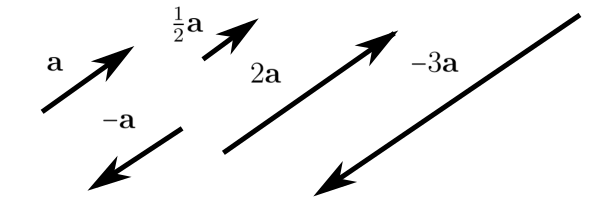
\includegraphics[width=0.7\linewidth]{figures/scalarProduct.pdf}
		\end{center}
		\caption{Produto por escalar.}
		\label{fig:scalarProduct}
	\end{figure}
\end{minipage}
\\

Por fim, também temos uma interpretação para um produto entre dois vetores, que chamamos de produto escalar. Essa operação associa dois elementos $\mathbf a, \mathbf b$ no espaço vetorial $E$ sobre $K$ com um elemento do corpo $K$ que é proporcional ao produto dos módulos de $\mathbf a$ e $\mathbf b$ e o cosseno do ângulo $\varphi$ entre estes dois vetores. Ou seja, $$\mathbf a \cdot \mathbf b = \norm{\mathbf a}\norm{\mathbf b}\cos \varphi,\quad \text{ com } 0\leq\varphi\leq 180^\circ.$$
Dessa forma, se o ângulo entre os vetores é 90$^\circ$ (i.e., são perpendiculares), $\mathbf a \cdot \mathbf b = 0$.\\

Com isso. estamos familiarizados com as noções de soma entre vetores (consequentemente com subtração), soma (subtração) e multiplicação (divisão) entre escalares, com a de multiplicação de um vetor por um escalar (resultando em vetor) e com a noção de multiplicação entre vetores (resultando em escalar). É intuitivo se perguntar se é possível multiplicar dois vetores e obter um vetor. De fato, esse vê-se um produto do tipo em álgebra linear, chamado de produto vetorial, mas ele é apenas definido sobre o $\mathbb{R}^3$. Agora iremos introduzir um novo produto entre vetores, chamado \textit{produto exterior}, mas primeiro precisaremos conhecer o que ele resultará.

\subsubsection{Bivetores}

\begin{figure}[H]
	\begin{center}
		\includegraphics[width=0.5\linewidth]{figures/2blade.pdf}
	\end{center}
	\caption{Áreas de superfícies planas $A$ e $A'$ nos respectivos planos $P$ e $P'$ \cite{lundholm2009clifford}.}
	\label{fig:2blade}
\end{figure}

Seja $A$ uma área de superfície plana em um plano $P$, dotada de um ``sentido'' (representado por uma flecha de rotação como na Figura~\ref{fig:2blade}). Se $A'$ representa outra área de superfície plana em outro plano $P'$, também dotada de um sentido, então pode-se definir a seguinte relação de equivalência: $A$ é equivalente a $A'$ se, e somente se, $P$ e $P'$ são paralelos, as áreas de $A$ e $A'$ são iguais e se os seus sentidos (de rotação) são o mesmo depois de transladar $A'$ em $A$ (ou seja, $P'$ para $P$). As classes de equivalência formadas por essas áreas orientadas de superfície plana são chamadas de \textit{$2$-vetor} (ou, um \textit{bivetor}).

Perceba que o bivetor $A$ (de qualquer formato) pode ser representado por um paralelogramo de lados $\mathbf a$ e $\mathbf b$ tais que a área orientada de superfície plana assim formada seja equivalente a $A$ (vide Figura~\ref{fig:2bladePlano}). A esse quadrilátero chamamos de \textit{produto exterior de $\mathbf a$ com $\mathbf b$} e escrevemos $\mathbf a \wedge \mathbf b$. Se a área de $A$ é zero, então escrevemos $A = 0$. Assim, $\mathbf a \wedge \mathbf a = 0$. Também, por $-A$ expressamos a classe de equivalência de todas as áreas orientadas de superfície plana com a mesma área e no mesmo plano que $A$, mas com um sentido de rotação contrário ao de $A$. Perceba que $-(\mathbf a \wedge \mathbf b) = \mathbf b \wedge \mathbf a$. Um \textit{bivetor unidade} é um bivetor $A$ com $\norm{A} = 1$.

	\begin{figure}[H]
		\begin{center}
			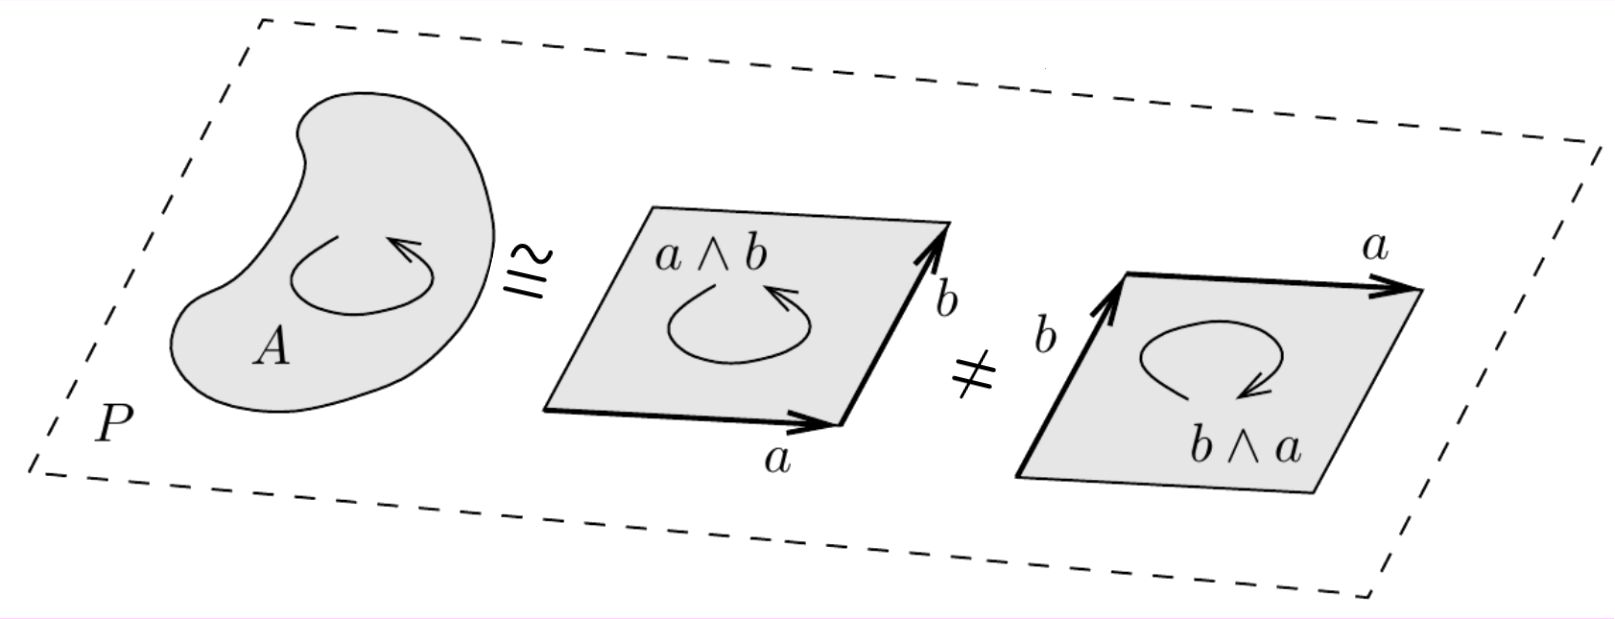
\includegraphics[width=0.75\linewidth]{figures/2bladePlano.pdf}
		\end{center}
		\caption{Um bivetor representado por um produto exterior $a\wedge b$ e $\mathbf b \wedge \mathbf a$ \cite{lundholm2009clifford}.}
		\label{fig:2bladePlano}
	\end{figure}

\subsubsection{Adição de bivetores}

A interpretação geométrica da adição de bivetores pode ser facilmente vista se existir um vetor comum entre os bivetores e, por sorte, em três dimensões sempre existe ao menos uma reta que intercepta dois planos quaisquer. Dessa forma, sejam $A = \mathbf a \wedge \mathbf c$ e $B = \mathbf b \wedge \mathbf c$ dois bivetores, então o bivetor $A + B$ é definido por $$A+B = \mathbf a \wedge \mathbf c + \mathbf b \wedge \mathbf c = (\mathbf a+ \mathbf b) \wedge \mathbf c.$$ 

\begin{figure}[H]
	\begin{center}
		\includegraphics[width=0.32\linewidth]{figures/2bladeSoma.pdf}
	\end{center}
	\caption{Interpretação geométrica da soma $A+B = (\mathbf a+\mathbf b)\wedge c$ \cite{lundholm2009clifford}.}
	\label{fig:2bladeSoma}
\end{figure}

Perceba que, como a soma de vetores é comutativa, $A+B = B+A$ e, portanto, o conjunto de bivetores sobre a adição forma um grupo abeliano. Bivetores também podem ser operados com escalares, donde eles se tornam um espaço vetorial. Descrevemos esse espaço por $\bigwedge^2\mathbb{R}^3$. Uma base para esse espaço vetorial pode ser construída usando a base $\{\mathbf e_1,\mathbf e_2,\mathbf e_3\}$ do espaço vetorial $\mathbb{R}^3$. As áreas orientadas de superfície plana obtidas através dos produtos exteriores $\mathbf e_1 \wedge \mathbf e_2, \mathbf e_1 \wedge \mathbf e_3, \mathbf e_2 \wedge \mathbf e_3$, entre os elementos da base de $\mathbb{R}^3$, formam uma base para o espaço vetorial $\bigwedge^2\mathbb{R}^3$.

\begin{minipage}{0.35\linewidth}
	\begin{figure}[H]
		\begin{center}
			\includegraphics[width=0.7\linewidth]{figures/bivectorsBase.pdf}
		\end{center}
		\caption{Base do $\bigwedge^2\mathbb{R}^3$ \cite{lounestoClifford}.}
		\label{fig:bivectorsBase}
	\end{figure}
\end{minipage}
\begin{minipage}{0.6\linewidth}
	\setlength\parindent{24pt} Assim, um bivetor arbitrário $B$ é uma combinação linear dos elementos da base: $$B = B_{1,2}\mathbf e_1\wedge \mathbf e_2 + B_{1,3}\mathbf e_1\wedge \mathbf e_3 + B_{2,3}\mathbf e_2\wedge \mathbf e_3,$$ e pode-se definir a norma (ou área) de $B$ como $$\norm{B} = \sqrt{B_{1,2}^2 + B_{1,3}^2 + B_{2,3}^2}.$$
\end{minipage}

\subsubsection{Trivetores}
O produto exterior $\mathbf a \wedge\mathbf b\wedge\mathbf c$ de três vetores $\mathbf a = a_1\mathbf e_1+a_2\mathbf e_2+a_3\mathbf e_3$, $\mathbf b = b_1\mathbf e_1+b_2\mathbf e_2+b_3\mathbf e_3$ e $\mathbf c = c_1\mathbf e_1+c_2\mathbf e_2+c_3\mathbf e_3$ representa o volume orientado do paralelepípedo com lados $\mathbf a$, $\mathbf b$ e $\mathbf c$: $$\mathbf a\wedge\mathbf b\wedge\mathbf c = \begin{tabular}{|c c c|}
	$a_1$&$a_2$&$a_3$\\
	$b_1$&$b_2$&$b_3$\\
	$c_1$&$c_2$&$c_3$
\end{tabular}
\ \mathbf e_1\wedge\mathbf e_2\wedge\mathbf e_3.
$$
Esse é um elemento do espaço vetorial unidimensional de trivetores (ou, 3-vetores) $\bigwedge^3\mathbb{R}^3$, com bases $\mathbf e_1\wedge\mathbf e_2\wedge\mathbf e_3$. O produto exterior é associativo, isso é, $$(\mathbf a\wedge \mathbf b)\wedge \mathbf c = \mathbf a\wedge (\mathbf b\wedge \mathbf c),$$ e antissimétrica: $$\mathbf a \wedge \mathbf b \wedge \mathbf c = \mathbf b \wedge \mathbf c \wedge \mathbf a = \mathbf c \wedge \mathbf a \wedge \mathbf b = -\mathbf c \wedge \mathbf b \wedge \mathbf a = - \mathbf a \wedge \mathbf c \wedge \mathbf b = -\mathbf b \wedge \mathbf a \wedge \mathbf c, \quad \forall a,b,c\in \mathbb{R}^3$$

O produto exterior dos elementos da base $\mathbf e_1,\mathbf e_2,\mathbf e_3$ do $\mathbb{R}^3$ é o volume orientado unitário $\mathbf e_1 \wedge\mathbf e_2 \wedge\mathbf e_3 \in \bigwedge^3\mathbb{R}^3$. O volume (ou norma) $\norm{\mathbf V}$ de um trivetor $\mathbf V = V\mathbf e_1\wedge\mathbf e_2\wedge\mathbf e_3$ é $\norm{V}$, isso é, $\norm{V\mathbf e_1\wedge\mathbf e_2\wedge\mathbf e_3} = V$ para $V\geq 0$ e $\norm{V\mathbf e_1\wedge\mathbf e_2\wedge\mathbf e_3} = -V$ para $V<0$.
\\

E agora podemos traçar uma relação entre aquele produto vetorial estudado em álgebra linear e o produto exterior de Grassmann. Sejam $\mathbf a = a_1\mathbf e_1+a_2\mathbf e_2 + a_3\mathbf e_3$ e $\mathbf b = b_1\mathbf e_1 + b_2\mathbf e_2 + b_3\mathbf e_3$ vetores. O bivetor $$\mathbf a \wedge\mathbf b = (a_2b_3 - a_3b_2)\mathbf e_2\wedge\mathbf e_3 + (a_3b_1 - a_1b_3)\mathbf e_3 \wedge\mathbf e_1 + (a_1b_2 - a_2b_1)\mathbf e_1\wedge\mathbf e_2$$ pode ser expresso como um ``determinante'' $$\mathbf a \wedge \mathbf b = 
\begin{tabular}{| c c c |}
	$\mathbf e_2 \wedge \mathbf e_3$& $\mathbf e_3 \wedge \mathbf e_1$& $\mathbf e_1 \wedge \mathbf e_2$\\
	$a_1$ &$a_2 $&$a_3 $\\
	$b_1 $&$b_2$ &$b_3 $
\end{tabular}.$$ E relembrando, define-se o \textit{produto vetorial de $\mathbf a$ por $\mathbf b$} como $$\mathbf a\times \mathbf b = (a_2b_3 - a_3b_2)\mathbf e_1 + (a_3b_1 - a_1b_3)\mathbf e_2+ (a_1b_2 - a_2b_1)\mathbf e_3,$$ que, por sua vez, pode ser representado pelo ``determinante'' $$\mathbf a \times \mathbf b = 
\begin{tabular}{| c c c |}
$\mathbf e_1$& $\mathbf e_2$& $\mathbf e_3$\\
$a_1$ &$a_2 $&$a_3 $\\
$b_1 $&$b_2$ &$b_3 $
\end{tabular}.$$

A interpretação geométrica de $\mathbf a\times \mathbf b$ é um vetor perpendicular ao plano de $\mathbf a\wedge\mathbf b$ e com norma igual ao volume do paralelepípedo formado por $\mathbf a$ e $\mathbf b$, isso é, $$\norm{\mathbf a\times\mathbf b} = \norm{\mathbf a \wedge \mathbf b} = \norm{\mathbf a}\norm{\mathbf b}\sin\varphi,$$ onde $0\leq\varphi\leq180^\circ$ é o ângulo entre $\mathbf a$ e $\mathbf b$.

\begin{figure}[H]
	\begin{center}
		\includegraphics[width=0.35\linewidth]{figures/produtoVetorial.pdf}
	\end{center}
	\caption{Interpretação geométrica de $\mathbf a \times \mathbf b$ \cite{lounestoClifford}.}
	\label{fig:produtoVetorial}
\end{figure}

\subsection{Álgebra Geométrica $\mathcal G(V,q)$}
A definição convencional de álgebra geométrica é sobre o contexto de espaços vetoriais monidos de produto interno, ou mais genericamente, uma \textit{forma quadrática}. No que se segue, considera-se um espaço vetorial $V$ de dimensão arbitrária sobre um corpo $K$.

\begin{definicao}[Forma quadrática]
Uma \textit{forma quadrática} $q$ sobre um espaço vetorial $V$ é um mapa $q: V\longrightarrow K$ tal que	
\begin{enumerate}
	\item $q(\alpha v) = \alpha^2q(v)$, para todo $\alpha\in K$ e $v\in V$; 
	\item o mapeamento $(v,w) \mapsto q(v+w) -q(v)-q(w)$ é linear em ambos $v$ e $w$.
\end{enumerate}
A forma bilinear correspondente $\beta_q(v,w):= \dfrac 1 2 (q(v+w)-q(v)-q(w))$ é chamada de \textit{polarização de q}.
\end{definicao}

Seja $$\mathcal{T}(V) := \bigoplus^\infty_{k=0}\bigoplus\, ^kV$$ descrevendo a álgebra tensorial sobre $V$, cujos elementos são somas finitas de tensores de grau arbitrário finito sobre $V$. Considere o ideal bilateral gerado por todos os elementos da forma $v\oplus v-q(v)$ de vetores $v$,
$$\mathcal{I}_q(V) := \{\sum_k A_k\oplus(v\oplus v-q(v))\oplus B_k \quad | \quad v\in V, \ A_k,B_k \in \mathcal{T}(V)\}.$$
Vamos definir a álgebra geométrica sobre $V$ através do quociente de $\mathcal{T}(V)$ por este ideal, de modo que, na álgebra resultante, a raiz de um vetor $v$ será igual ao escalar $q(v)$, como segue.

\begin{definicao}[Álgebra geométrica]
	A \textit{álgebra geométrica} $\mathcal{G}(V,q)$ sobre o espaço vetorial $V$ com forma quadrática $q$ é definido por $$\mathcal{G}(V,q) := \mathcal{T}(V)/\mathcal{I}_q(V).$$
\end{definicao}

\begin{observacao}[Notação]
	Quando for claro o contexto que estivermos trabalhando com o espaço vetorial $V$ ou a forma quadrática $q$, iremos suprimi-los da notação, ficando apenas com $\mathcal{G}(V)$ ou simplesmente $\mathcal{G}$.
\end{observacao}

O produto em $\mathcal{G}$ é chamado de \textit{produto geométrico} ou \textit{produto de Clifford}, é herdado do produto tensorial em $\mathcal{T}(V)$ e iremos descrevê-lo por $$\mathcal{G}\times \mathcal{G}\rightarrow\mathcal{G},\quad \quad \quad\quad \quad \quad\quad \quad\quad \quad\ \ $$$$(A,B)\mapsto AB:= [A\oplus B] = A\oplus
 B+\mathcal{I}_q.$$
 
Perceba que esse produto é bilinear e associativo. Além disso, $$v^2 = [v\oplus v] = [v\oplus v-q(v)1] + q(v)1_\mathcal{G} = q(v)$$ e $$q(v+w) = (v+w)^2 = v^2 + vw + wv + w^2 = q(v) + vw + wv + q(w),$$
de modo que, juntos com a definição de $\beta_q$, encontra-se as seguintes identidades sobre $\mathcal{G}$ para todo $v,w \in V$: $$v^2 = q(v)\quad \text{ e } \quad vw+wv = 2\beta_q(v,w).$$

\begin{proposicao}[Universalidade]
	
\end{proposicao} 
 
\subsection{O produto de Clifford}

Temos o objetivo de definir uma operação de produto de vetores que se comporte de forma parecida com o produto de um corpo, isto é, que respeite, $\forall a,b,c \in \mathbb{R}$, os seguintes axiomas
\begin{enumerate}
	\item \emph{(Comutatividade).} $ab = ba;$
	\item \emph{(Associatividade).} $a(bc)=(ab)c;$
	\item \emph{(Distributividade).} $a(b+c)=ab+ac;$
	\item \emph{(Preservação da norma).} $|\,ab\,| = |\,a\,||\,b\,|.$
\end{enumerate}

Os números complexos satisfazem isso. Porém, como isso não é possível para dimensões maiores \cite{lounestoClifford}, teremos de abrir mão de alguma propriedade. Abriremos mão da comutatividade.

\begin{definicao}[Produto de Clifford]
	Sejam dois versores ortogonais $\mathbf{e_1}$ e $\mathbf{e_2}$ no $\mathbb{R}^2$. Para dois vetores $\mathbf{a}$ = $a_1\mathbf{e_1} + a_2\mathbf{e_2}$ e $\mathbf b = b_1\mathbf{e_1} + b_2\mathbf{e_2}$, o \emph{produto de Clifford} $\mathbf{ab}$ é definido como $$\mathbf{ab} = a_1b_1 + a_2b_2 + (a_1b_2-a_2b_1)\mathbf{e_{12}},$$
	isto é, a soma de um escalar com um bivetor.
\end{definicao}



Perceba que pode-se separar as duas partes do produto de Clifford como $$\mathbf{a\cdot b} + \mathbf{a \wedge b} \ = \ a_1b_1 + a_2b_2 + (a_1b_2 - a_2b_1)\mathbf{e_{12}}.$$

\subsection{Álgebra dos Quatérnios}
William Rowan Hamilton fora uma criança extremamente precoce. De origem irlandesa, viveu entre 1805 e 1865, onde, aos três anos de idade lia perfeitamente inglês. Devido a morte antecipada de seus pais teve como orientador um tio linguista e aos cinco anos sabia latim e hebraico. Até os dez anos já era familiarizado com italiano, francês, árabe, sânscrito, persa, caldeu e algumas outras línguas orientais. Ainda criança, Hamilton demonstrou grande interesse pela matemática, influenciado por autores como Newton e Laplace, caminhava a passos largos para o mundo da física e astronomia. Sem dúvidas estava florescendo um dos grandes nomes da ciência do século XIX. \cite{BoyerMathHistory,AlgebraAbstrata2BienalSBM}

Porém, nos atentando as suas contribuições à matemática, tudo começou quando Hamilton percebeu que uma notação utilizada na teoria dos números complexos não era a mais adequada. Ele percebeu que a expressão $a + bi$ não era realmente uma soma, isto é, não é como somar dois números reais que pertencem a mesma dimensão, o que dá sentido a soma. Ele afirma que o sinal ‘$+$’ é um equívoco, um acidente histórico, e que as duas partes não podem ser naturalmente somadas. A partir deste pensamento construiu e publicou em 1833 a teoria de números complexos formalmente como conhecemos hoje, definindo a soma e produto em pares ordenados, ou seja:
\begin{equation*}
	(a,b) + (c,d) = (a + b, c + d)
\end{equation*}
\begin{equation*}
	(a, b)(c, d) = (ac-bd, ad + bc)
\end{equation*}

Claramente Hamilton só pode perceber isso devido sua inclinação física, afinal, físicos adoram se perguntar sobre as dimensões do que se está somando. Graças também a esta inclinação Hamilton logo percebeu como esta nova abordagem permitiria uma visão dos números complexos como entidades orientadas no plano e, maravilhado com as possibilidades de sua descoberta, não demorou muito para que se perguntasse como seria esta relação se fosse expandida para o espaço tridimensional. Infelizmente as respostas não foram fáceis e por dez anos trabalhou arduamente tentando desenvolver ternas (três representantes do espaço) que pudessem ser multiplicadas, tendo em vista que a soma e a subtração se davam trivialmente. A demonstração de que Hamilton nunca conseguiria sua terna encontra-se em \cite{QuaterniosJucineide}. 

Tais questões manteriam-se obscuras se não fosse pelo histórico dia de 16 de outubro de 1843, onde Hamilton, andando ao lado de sua esposa na ponte Brougham sobre o Royal Canal para presidir uma reunião do Conselho da Real Sociedade da Irlanda, dividia-se entre conversas ocasionais e no pensar sobre seu trabalho e tão logo teve um \textit{insight}: Percebeu que seus problemas sumiriam se utilizasse quádruplas em vez de ternas e ignorasse a comutatividade para a multiplicação. Percebeu que para quádruplas $a + bi + cj + dk$ teria $i^2 = j^2 = k^2 = ijk = -1$. Desta fórmula fundamental tira-se a solução do problema da multiplicação que Hamilton encontrara, a origem da Regra de Fleming (vulgarmente conhecida como “regra da mão direita”) e, entre outras coisas surpreendentes, uma nova álgebra que iria contra os princípios matemáticos da época: \textit{A Álgebra dos Quatérnios}.

\textbf{Definição: }Seja $B_{\mathbb{R}^3}=\{i,j,k\}$ a base canônica de $\mathbb{R}^3$. Um \textit{quatérnio} é definido como um elemento da forma 
\begin{equation}
	q=q_0+\mathbf{q_v},
\end{equation} 
onde $q_0 \in \mathbb{R}$ é um escalar e $\mathbf{qv}=q_1\mathbf{i}+q_2\mathbf{j}+q_3\mathbf{k}$ é um vetor de $\mathbb{R}^3$.
\\

Ou seja, todo elemento $q$ da forma $q = q_0 + q_1\textbf{i} + q_2\textbf{j} + q_3\textbf{k}$ é um quatérnio e a medida que variamos os valores dos coeficientes reais $q_0, q_1, q_2$ e $q_3$ independentemente uns dos outros na reta real percorremos todos os quatérnios possíveis, nos levando a criação do \textit{Conjunto dos Quatérnios}, definido por $\mathbb{H}$. Perceba então que há uma relação biunívoca entre $\mathbb{H}$ e $\mathbb{R}^4$, uma vez que um quatérnio pode ser escrito como a quádrupla $q = (q_0, q_1, q_2, q_3) \in \mathbb{R}^4$. \cite{fidalgotese}
\\

\textbf{Definição:} Seja $B_\mathbb{H} = \{1, \mathbf{i}, \mathbf{j}, \mathbf{k}\}$ definida como a \textit{base canônica de $\mathbb{H}$} tal que $\mathbf{i}^2 = \mathbf{j}^2 = \mathbf{k}^2 = \mathbf{ijk} = -1$.
\\

Pode-se tratar agora de operações aritméticas no Conjunto dos Quatérnios:
\phantomsection
\addcontentsline{toc}{subsubsection}{Operações sobre $\mathbb{H}$}
\begin{itemize}
	\item \textbf{Adição:} dados dois quatérnios $p=p_0+\mathbf{p_v}$ e $q=q_0+\mathbf{q_v}$ em $\mathbb{H}$, define-se a adição de $p$ a $q$ como  
	\begin{equation}
		p+q=(p_0+q_0)+(\mathbf{p_v}+\mathbf{q_v})
	\end{equation}
	Temos uma proposição que mostra que esta adição está bem-definida no conjunto de quatérnios. 
	\\ \newline \textbf{Proposição:} \textit{O conjunto $\mathbb{H}$ é fechado para adição}.
	\\ \newline \textit{Demonstração.} O que queremos mostrar é que a soma de dois quatérnios é, por sua vez, um novo quatérnio. De fato: considerando $r=p+q$, podemos escrever o elemento $r$ como
	\begin{equation}
		r=r_0+\mathbf{r_v}
	\end{equation}
	onde sua parte escalar é dada por $r_0=p_0+q_0$ e sua parte vetorial é dada por $\mathbf{r_v=p_v+q_v}. \hfill\blacksquare$
	\\ \newline Dados $p,q,r \in \mathbb{H}$ arbitrários, temos as seguintes propriedades para a adição de quatérnios.
	\begin{enumerate}
		\item \textbf{Associatividade:} $(p+q)+r=p+(q+r)$.
		\\ \newline \textit{Demonstração.} Seja $p=p_0+\mathbf{p_v}, q=q_0+\mathbf{q_v}, r=r_0+\mathbf{r_v}$,\,\,tal que $p,q,r \in \mathbb{H}$. Partindo de $(p+q)+r$ \,\,temos:
		\\ \newline $(p+q)+r=[(p_0+\mathbf{p_v})+(q_0+\mathbf{p_v})]+(r_0+\mathbf{r_v})=[(p_0+q_0)+(\mathbf{p_v}+\mathbf{q_v})]+(r_0+\mathbf{r_v})=[(p_0+q_0+r_0)+(\mathbf{p_v}+\mathbf{q_v}+\mathbf{r_v})]=[(p_0+q_0+r_0)+(\mathbf{p_v}+\mathbf{q_v}+\mathbf{r_v})]=\{[p_0+(q_0+r_0)]+[\mathbf{p_v}+(\mathbf{q_v}+\mathbf{r_v})]\}=(p_0+\mathbf{p_v})+[(q_0+r_0)+(\mathbf{q_v}+\mathbf{r_v})]=(p_0+\mathbf{p_v})+[(q_0+\mathbf{q_v})+(r_0+\mathbf{r_v})]=p+(q+r). \hfill\blacksquare$
		\\ \item \textbf{Comutatividade:} $p+q=q+p$
		\\ \newline \textit{Demonstração.} Seja $p=p_0+\mathbf{p_v}, q=q_0+\mathbf{q_v}$,\,\,tal que $p,q \in \mathbb{H}$. Partindo de $p+q$, temos:
		\\ \newline $p+q=(p_0+\mathbf{p_v})+(q_0+\mathbf{q_v})=(p_0+q_0)+(\mathbf{p_v}+\mathbf{q_v})=(q_0+p_0)+(\mathbf{q_v}+\mathbf{p_v})=q+p.\hfill\blacksquare$
		\\ \item \textbf{Existência de Elemento Neutro:} Existe um elemento neutro, a saber, $0_{\mathbb{H}}=0+\mathbf{0_v} \in \mathbb{H}$, de modo que,
		\begin{equation}
			p+0_{\mathbb{H}}=0+p=p
		\end{equation}
		\\ \textit{Demonstração.}  Seja $p=p_0+\mathbf{p_v} \textrm{ e } 0_{\mathbb{H}}=0+\mathbf{0_v}$,\,\,tal que $p,0_{\mathbb{H}} \in \mathbb{H}$. Partindo de $p+0_{\mathbb{H}}$, temos:
		\\ \newline $p+0_{\mathbb{H}}=(p_0+\mathbf{p_v})+(0+\mathbf{0_v})=(p_0+0)+(\mathbf{p_v}+\mathbf{0_v})=(0+p_0)+(\mathbf{0_v}+\mathbf{p_v})=p_0+\mathbf{p_v}=p.\hfill\blacksquare$
		\\ \item \textbf{Existência de Elemento Oposto:} Existe um elemento oposto para cada $p=p_0+\mathbf{p_v} \in \mathbb{H}$, dado por $-p=-p_0-\mathbf{p_v}$, de modo que sua soma com $p$ resulte no elemento neutro da adição do item anterior, ou seja,
		\begin{equation}
			p+(-p)=(-p)+p=0_{\mathbb{H}}
		\end{equation}
		\\ \textit{Demonstração.} De fato, se partirmos de $p+(-p)$, temos:
		\\ \newline $p+(-p)= (p_0+\mathbf{p_v})+(-p_0-\mathbf{p_v})=[p_0+(-p_0)]+[\mathbf{p_v}+(\mathbf{-p_v})]=(p_0-p_0)+(\mathbf{p_v}-\mathbf{p_v})=0+\mathbf{0_v}=0_{\mathbb{H}}.\hfill\blacksquare$
	\end{enumerate}
	Como a adição de quatérnios satisfaz estas propriedades, temos o seguinte resultado.
	\\ \newline \textbf{Proposição: } ($\mathbb{H},+$) é um \textit{grupo abeliano}.
	\\
	
	\item \textbf{Multiplicação por Escalar:} Dado um quatérnio $q=q_0+\mathbf{q_v} \in \mathbb{H}$ e uma constante escalar real $\alpha \in \mathbb{R}$, define-se a multiplicação de $q$ pelo escalar $\alpha$ da forma
	\begin{equation}
		\alpha q=(\alpha q_0)+(\alpha \mathbf{q_v})
	\end{equation}
	A próxima proposição mostra que esta operação, unindo itens de espaços distintos, está bem definida no conjunto dos quatérnios.
	\\ \newline \textbf{Proposição:} O \textit{conjunto $\mathbb{H}$ é fechado para a multiplicação de escalares reais.}
	\\ \textit{Demonstração.} Queremos demonstrar que a multiplicação de um escalar por um quatérnio tem por resultado um novo quatérnio. Com efeito: podemos considerar tal multiplicação como o elemento 
	\begin{equation*}
		r=r_0+\mathbf{r_v}
	\end{equation*}
	onde sua parte escalar é dada por $r_0=\alpha q_0 \in \mathbb{R}$ e sua parte vetorial é dada por $\mathbf{r_v}=\alpha \mathbf{q_v} \in \mathbb{R}^3.\hfill\blacksquare$
	\\ \newline A multiplicação por escalar também tem uma série de propriedades. Dados os números reais $\alpha,\beta$ e os quatérnios $p$ e $q$, temos:
	\begin{enumerate}
		\item \textbf{Associatividade:} $(\alpha \beta)q=\alpha(\beta q)$ 
		\\ \newline \textit{Demonstração.} De fato, seja $\alpha, \beta \in \mathbb{R}$ e $q=q_00+\mathbf{q_v} \in \mathbb{H}$, partindo de $(\alpha \beta)q$ temos:
		\\ \newline $(\alpha \beta)q=(\alpha \beta)(q_0+\mathbf{q_v})=\alpha \beta q_0+\alpha \beta \mathbf{q_v}=\alpha(\beta q_0+\beta \mathbf{q_v})=\alpha(\beta q).\hfill\blacksquare$
		\\ \item \textbf{Multiplicação pela Unidade:} $1q=q$
		\\ \newline \textit{Demonstração.} Queremos provar que $1q=q$. Para isto, tome $\alpha \in \mathbb{R}$, com $\alpha = 1$. Partindo de $1q=1(q_0+\mathbf{q_v})=(1q_0+1\mathbf{q_v})=q_0+\mathbf{q_v}=q$. Logo, $1q=q.\hfill\blacksquare$
		\\ \item \textbf{Distributividade em relação à soma:} estas duas propriedades unem a adição e a multiplicação por escalar e são dadas por
		\begin{equation*}
			(\alpha+\beta)q=\alpha q + \beta q
		\end{equation*}e \begin{equation*}
			\alpha(p+q)=\alpha p + \alpha q	
		\end{equation*}
		\\ \textit{Demonstração.} Seja $\alpha,\beta \in \mathbb{R}$ e $p,q \in \mathbb{H}$. Partindo de $(\alpha + \beta)q=((\alpha + \beta)q_0 + (\alpha + \beta)\mathbf{q_v})$. Deste modo, é fácil ver que $((\alpha + \beta)q_0 + (\alpha + \beta)\mathbf{q_v})=\alpha(q_0+\mathbf{q_v})+\beta(q_0+\mathbf{q_v})=\alpha q+\beta q$. Analogamente, se olharmos para $\alpha q+\beta q$. Agora, partindo de $\alpha(p+q)=\alpha p+\alpha q$. Aplicando as devidas distributividades, temos que $\alpha p+\alpha q=(\alpha p_0+\alpha\mathbf{p_v})+(\alpha q_0+\alpha\mathbf{q_v})=\alpha p+\alpha q$. Analogamente para $\alpha p+\alpha q$. Portanto, a distributividade é válida. \hfill$\blacksquare$ 
	\end{enumerate}
\end{itemize}

Sabendo do isomorfismo já citado entre $\mathbb{H}$ e $\mathbb{R}^4$ e percebendo que as operações descritas preservam as mesmas operações entre os dois conjuntos, nota-se que existe uma relação de isomorfismo entre $\mathbb{H}$ e $\mathbb{R}^4$. Isso se deve ao fato de que o calculo vetorial como conhecemos hoje é mera simplificação das ideias de Hamilton sobre quatérnios, simplificação feita por Josiah Willard Gibbs (1839 – 1903) em um conjunto de notas para seus estudantes de física-matemática intitulado Elements of Vector Analysis \cite{AlgebraAbstrata2BienalSBM}.

\textbf{Proposição:} O espaço vetorial dos quatérnios $\mathbb{H}$ é isomorfo ao espaço vetorial Euclidiano de dimensão 4, i.e. $\mathbb{H} \simeq \mathbb{R}^4$.
\\

Assim como os complexos, os quatérnios também tem conjugado. E esses são definidos da seguinte forma:

\textbf{Definição:} Seja $q = q_0 + \mathbf{q_v} \in \mathbb{H}$, define-se seu \textit{conjugado} como $q^* = q_0 - \mathbf{q_v}$.
\\

\phantomsection
\addcontentsline{toc}{subsubsection}{Produto algébrico dos quatérnios}
Tendo as definições já estabelecidas, pode-se construir a terceira operação dos quatérnios, baseando-se em \cite{QuaterniosAndRotationsKuipers}, justamente a que causou dez anos de trabalho para Hamilton e que torna sua álgebra um tanto não trivial, o \textit{produto algébrico dos quatérnios}:

Suponha dois elementos pertencentes a $\mathbb{H}/0$, $p = p_0 + \mathbf{p_v}$ e $q = q_0 + \mathbf{q_v}$ e escritos em $B_{\mathbb{H}}$. Sabe-se que podemos escrever $\mathbf{p_v} = p_1\mathbf{i} + p_2\mathbf{j} + p_3\mathbf{k}$ e $\mathbf{q_v} = q_1\mathbf{i} + q_2\mathbf{j} + q_3\mathbf{k}$. Se multiplicarmos os dois elementos termo a termo, como na propriedade distributiva, teremos:
\begin{equation}
	\begin{aligned}
		pq = (p_0+\mathbf{i}p_1+\mathbf{j}p_2+\mathbf{k}p_3)(q_0+\mathbf{i}q_1+\mathbf{j}q_2+\mathbf{k}q_3) \\ = (p_0q_0+p_0+\mathbf{i}p_0q_1+p_1q_0)+\mathbf{j}(p_0q_2+p_2q_0) \\ +\mathbf{k}(p_0q_3+p_3q_0)+\mathbf{i}^2p_1q_1+\mathbf{j}^2p_2q_2+\mathbf{k}^2p_3q_3+\mathbf{ij}p_1q_2+\mathbf{ji}p_2q_1 \\ +\mathbf{ik}p_1q_3+\mathbf{ki}p_3q_1+\mathbf{jk}p_2q_3+\mathbf{kj}p_3q_2
	\end{aligned}		   	       
\end{equation}
Mas podemos utilizar de algumas definições para simplificar a equação acima. Os produtos dos versores a seguir foram definidos por Hamilton por construção a partir de seus três planos retangulares intersectados utilizando de rotações \cite{QuaterniosHamilton}.
\begin{equation*}
	\mathbf{ij} = \mathbf{k} = \mathbf{-ji}
\end{equation*}
\begin{equation*}
	\mathbf{jk} = \mathbf{i} = \mathbf{-kj}
\end{equation*}
\begin{equation*}
	\mathbf{ki} = \mathbf{j} = \mathbf{-ik}
\end{equation*}
Note que esses são os produtos que fazem com que esta álgebra seja não comutativa no produto. Também são graças a esses produtos que poderemos agrupar os termos comuns em 1. Logo, usando os produtos definidos acima e a fórmula fundamental $\mathbf{i}^2 = \mathbf{j}^2 = \mathbf{k}^2 = \mathbf{ijk} = -1$ temos:
\begin{equation}
	\begin{aligned}
		pq = (p_0q_0-p_1q_1+p_2q_2+p_3q_3)+p_0(\mathbf{i}q_1+\mathbf{j}q_2+\mathbf{k}q_3+q_0(\mathbf{i}p_1+\mathbf{j}p_2+\mathbf{k}p_3) \\ +\mathbf{i}(p_2q_3-p_3q_2)+\mathbf{j}(p_3q_1-p_1q_3)+\mathbf{k}(p_1q_2-p_2q_1).
	\end{aligned}
\end{equation}
Veja que conseguimos um produto interno no $\mathbb{R}^3$, uma vez que $<\mathbf{pv}, \mathbf{qv}> = p_1q_1 + p_2q_2 + p_3q_3$, então, por uma questão de estética, para deixar está operação menor:
\begin{equation}
	\begin{aligned}
		pq = p_0q_0-<\mathbf{pv,qv}>+p_0\mathbf{q_v}+q_0\mathbf{p_v}+\mathbf{i}(p_2p_3-p_3p_2)+\mathbf{j}(p_3q_1-p_1q_3)\\+\mathbf{k}(p_1q_2-p_2q_1)
	\end{aligned}
\end{equation}
Mais uma vez podemos simplificar esta equação, porém agora utilizando do produto vetorial no $\mathbb{R}^3$. Sabendo que $\mathbf{p_v} \times \mathbf{q_v} = \mathbf{i}(p_2q_3 - p_3q_2) + \mathbf{j}(p_3q_1 - p_1q_3) + \mathbf{k}(p_1q_2 - p_2q_1)$. Assim, chegamos ao produto algébrico de quatérnios, dado por:
\begin{equation*}
	pq=p_0q_0-<\mathbf{p_v,q_v}>+p_0\mathbf{q_v}+q_0\mathbf{p_v}+\mathbf{p_v}\times\mathbf{q_v}
\end{equation*}

Agora, formalmente.

\textbf{Definição} (Produto Algébrico de Quatérnios). Dados dois quatérnios não nulos $p,q \in \mathbb{H}/0$, o produto algébrico entre $p$ e $q$ é dado por 
\begin{equation}
	pq=p_0q_0-<\mathbf{p_v,q_v}>+p_0\mathbf{q_v}+q_0\mathbf{p_v}+\mathbf{p_v}\times\mathbf{q_v}
\end{equation}
Considerando $p=p_0+\mathbf{p_v}$ e $q=q_0+\mathbf{q_v}$.

\textbf{Proposição:} O conjunto dos quatérnios é fechado pelo produto algébrico de quatérnios.
\\ \newline \textit{Demonstração.} De fato. Considerando a equação (11), temos que o quatérnio produto algébrico $r=pq$ pode ser escrito como 
\begin{equation}
	r=r_0+\mathbf{r_v},
\end{equation}
onde $r_0=(p_0q_0-<\mathbf{p_v,q_v}>)$ e $\mathbf{r_v}=(p_0\mathbf{q_v}+q_0\mathbf{p_v}+\mathbf{p_v}\times\mathbf{q_v})$. Portanto, $r \in \mathbb{H} \hfill\blacksquare$
\\ 

\textbf{Proposição:} O produto algébrico de quatérnios é associativo. Ou seja, dados $p,q,r \in \mathbb{H}$, temos que 
\begin{equation}
	(pq)r=p(qr)
\end{equation}
\\ \textbf{Proposição:} O produto algébrico de quatérnios é distributivo em relação à adição, ou seja, $p,q,r \in \mathbb{H}$
\begin{equation}
	p(q+r)=pq+pr \,\,\,\,\,\,\,\,e\,\,\,\,\,\,\,\, (p+q)r=pr+qr
\end{equation}
\\

Temos então o conjunto dos quatérnios monido das operações de adição, multiplicação por escalar e do produto de quatérnios, o que forma uma álgebra associativa, denominada \textit{Álgebra dos Quatérnios}. Construída tal álgebra, pode-se definir algumas propriedades interessantes.
\\

\textbf{Proposição:} Seja $1_\mathbb{H} = 1 + \mathbf{0_v} \in \mathbb{H}$ o elemento da álgebra dos quatérnios definido como identidade do produto de quatérnios. Isto é, para todo $q = q_0 + \mathbf{q_v} \in \mathbb{H}$, $q1_\mathbb{H} = q$.
\\

Como já definiu-se produto de quatérnios e conjugado, pode-se definir a norma de um quatérnio, seu tamanho:

\textbf{Definição:} Dado $q \in \mathbb{H}$, sua \textit{norma} é dada por $N(q) = \sqrt[]{q^*q}$. 

Duas propriedades para normas de quatérnios seguem. 
\\

\textbf{Proposição:} Dado $p \in \mathbb{H}$, a norma do conjugado de $p$ é igual a sua própria norma, ou seja, $N(p^*) = N(p)$.
\\

\textbf{Proposição:} Sejam $p, q \in \mathbb{H}$, a norma do produto $pq$ é igual ao produto das normas de $p$ e $q$, isto é, $N(pq) = N(p)N(q)$.
\\

\phantomsection
\addcontentsline{toc}{chapter}{Referências Bibliográficas}

\bibliographystyle{unsrt}
\bibliography{references}

\end{document}
